\documentclass[journal]{IEEEtran}
\usepackage{cite}
\usepackage{amsmath,amssymb,amsfonts}
\usepackage{graphicx}
\usepackage{textcomp}
\usepackage{xcolor}
\usepackage{booktabs}
\usepackage{url}
\usepackage{array}
\usepackage{siunitx}
% AUTO-GENERATED by Paper/generate_paper_assets.py from results/final/*.json - do not edit by hand
\newcommand{\nRaw}{572}
\newcommand{\nRawPatients}{500}
\newcommand{\nClinical}{493}
\newcommand{\nClinicalPos}{305}
\newcommand{\nMatched}{347}
\newcommand{\nMatchedPos}{237}
\newcommand{\nTrain}{277}
\newcommand{\nTest}{70}
\newcommand{\nProteinSamples}{352}
\newcommand{\nProteinRaw}{487}
\newcommand{\nProteinKept}{456}
\newcommand{\nPCAll}{129}
\newcommand{\nEvents}{9}
\newcommand{\nEventsTrain}{8}
\newcommand{\nEventsTest}{1}
\newcommand{\nEventsAll}{12}
\newcommand{\nFeatFull}{18}
\newcommand{\nFeatPreop}{13}
\newcommand{\nSites}{9}
\newcommand{\nSiteTotal}{384}
\newcommand{\nExternal}{109}
\newcommand{\bpLOC}{0.775}
\newcommand{\bpFL}{0.790}
\newcommand{\bpFR}{0.782}
\newcommand{\bpCEN}{0.789}
\newcommand{\bpBL}{0.723}
\newcommand{\bpFLminusLOC}{+0.015\ [\ensuremath{-}0.007, +0.037]}
\newcommand{\bpFRminusFL}{\ensuremath{-}0.008\ [\ensuremath{-}0.013, \ensuremath{-}0.003]}
\newcommand{\bpCENminusFL}{\ensuremath{-}0.001\ [\ensuremath{-}0.004, +0.002]}
\newcommand{\bpFLminusBL}{+0.067\ [+0.048, +0.086]}
\newcommand{\bpLcPartOne}{0.696}
\newcommand{\bpLcFrOne}{0.751}
\newcommand{\bpLcPartAll}{0.838}
\newcommand{\bpLcFrAll}{0.785}
\newcommand{\bpLooShapRho}{0.48\ [0.34, 0.62]}
\newcommand{\bpShapSizeRho}{0.51}
\newcommand{\bpMacroSites}{7.4}
\newcommand{\cvFull}{0.818}
\newcommand{\cvPreop}{0.642}
\newcommand{\cvProt}{0.574}
\newcommand{\cvFullProt}{0.659}
\newcommand{\cvSkFull}{0.824}
\newcommand{\cvRFFullProt}{0.782}
\newcommand{\cvRFFull}{0.803}
\newcommand{\cvProtDiff}{\ensuremath{-}0.159\ [\ensuremath{-}0.188, \ensuremath{-}0.130]}
\newcommand{\cvPreopDiff}{+0.176\ [+0.148, +0.203]}
\newcommand{\cvProtPreopDiff}{\ensuremath{-}0.047\ [\ensuremath{-}0.080, \ensuremath{-}0.013]}
\newcommand{\nFolds}{25}
\newcommand{\driftRedMin}{32.0}
\newcommand{\driftRedMax}{36.4}
\newcommand{\driftAvgIID}{0.206}
\newcommand{\driftAvgSkew}{0.770}
\newcommand{\driftMuZero}{0.599}
\newcommand{\driftMuOne}{0.268}
\newcommand{\sigmaTen}{5.68}
\newcommand{\sigmaFive}{10.55}
\newcommand{\sigmaTwo}{24.99}
\newcommand{\sigmaOne}{49.02}
\newcommand{\sigmaHalf}{97.01}
\newcommand{\auNoDP}{0.823}
\newcommand{\auAvgTen}{0.821}
\newcommand{\auProxTen}{0.823}
\newcommand{\auLossTen}{\ensuremath{-}0.002\ [\ensuremath{-}0.009, +0.005]}
\newcommand{\auAvgFive}{0.818}
\newcommand{\auProxFive}{0.821}
\newcommand{\auLossFive}{\ensuremath{-}0.005\ [\ensuremath{-}0.014, +0.003]}
\newcommand{\auAvgTwo}{0.800}
\newcommand{\auProxTwo}{0.812}
\newcommand{\auLossTwo}{\ensuremath{-}0.023\ [\ensuremath{-}0.038, \ensuremath{-}0.008]}
\newcommand{\auAvgOne}{0.761}
\newcommand{\auProxOne}{0.789}
\newcommand{\auLossOne}{\ensuremath{-}0.063\ [\ensuremath{-}0.087, \ensuremath{-}0.038]}
\newcommand{\auAvgHalf}{0.691}
\newcommand{\auProxHalf}{0.720}
\newcommand{\auLossHalf}{\ensuremath{-}0.132\ [\ensuremath{-}0.180, \ensuremath{-}0.085]}
\newcommand{\gridSup}{12}
\newcommand{\gridCells}{20}
\newcommand{\gridSupCtl}{3}
\newcommand{\gridNoDPmax}{0.0019}
\newcommand{\gridOneHalfMin}{0.028}
\newcommand{\gridOneHalfMax}{0.030}
\newcommand{\gridCtlOneHalfMax}{0.003}
\newcommand{\pflLocalThree}{0.754}
\newcommand{\pflProxThree}{0.811}
\newcommand{\pflPFLThree}{0.805}
\newcommand{\pflGainThree}{+0.051\ [+0.015, +0.086]}
\newcommand{\pflVsProxThree}{\ensuremath{-}0.006\ [\ensuremath{-}0.022, +0.011]}
\newcommand{\pflLocalFive}{0.796}
\newcommand{\pflProxFive}{0.817}
\newcommand{\pflPFLFive}{0.814}
\newcommand{\pflGainFive}{+0.018\ [\ensuremath{-}0.021, +0.057]}
\newcommand{\pflVsProxFive}{\ensuremath{-}0.003\ [\ensuremath{-}0.011, +0.005]}
\newcommand{\pflLocalTen}{0.785}
\newcommand{\pflProxTen}{0.841}
\newcommand{\pflPFLTen}{0.838}
\newcommand{\pflGainTen}{+0.053\ [+0.010, +0.096]}
\newcommand{\pflVsProxTen}{\ensuremath{-}0.003\ [\ensuremath{-}0.014, +0.007]}
\newcommand{\shRhoTenThree}{0.68}
\newcommand{\shRhoHalfThree}{0.25}
\newcommand{\shTSTenThree}{0.79}
\newcommand{\shTSHalfThree}{0.51}
\newcommand{\shRRHalfThree}{0.57}
\newcommand{\shLooThree}{0.68\ [0.42, 0.93]}
\newcommand{\shSizeThree}{0.55\ [0.31, 0.79]}
\newcommand{\shRThree}{5}
\newcommand{\shRhoTenFive}{0.66}
\newcommand{\shRhoHalfFive}{0.30}
\newcommand{\shTSTenFive}{0.65}
\newcommand{\shTSHalfFive}{0.41}
\newcommand{\shRRHalfFive}{0.74}
\newcommand{\shLooFive}{0.34\ [0.14, 0.54]}
\newcommand{\shSizeFive}{0.33\ [0.11, 0.55]}
\newcommand{\shRFive}{5}
\newcommand{\shRhoTenTen}{0.73}
\newcommand{\shRhoHalfTen}{0.36}
\newcommand{\shTSTenTen}{0.62}
\newcommand{\shTSHalfTen}{0.30}
\newcommand{\shRRHalfTen}{0.88}
\newcommand{\shLooTen}{0.44\ [0.30, 0.58]}
\newcommand{\shSizeTen}{0.46\ [0.35, 0.58]}
\newcommand{\shRTen}{2}
\newcommand{\miaNoDP}{0.511\ [0.489, 0.533]}
\newcommand{\miaOne}{0.510\ [0.484, 0.537]}
\newcommand{\miaHalf}{0.512\ [0.490, 0.534]}
\newcommand{\miaCtl}{0.659\ [0.640, 0.678]}
\newcommand{\miaGap}{+0.017\ [\ensuremath{-}0.007, +0.041]}
\newcommand{\shiftCovTwo}{0.765}
\newcommand{\shiftConTwo}{0.498}
\newcommand{\shiftBase}{0.826}
\newcommand{\abCen}{0.823}
\newcommand{\abAvg}{0.824}
\newcommand{\abProx}{0.826}
\newcommand{\abDPFive}{0.820}
\newcommand{\abDPOne}{0.787}
\newcommand{\abPreop}{0.659}
\newcommand{\abProt}{0.682}
\newcommand{\pNineN}{5{,}610}
\newcommand{\pNinePos}{2{,}146}
\newcommand{\pNineHosp}{19}
\newcommand{\pNineCountries}{8}
\newcommand{\pNinePrevLo}{12}
\newcommand{\pNinePrevHi}{60}
\newcommand{\pNinePrev}{38.3}
\newcommand{\pNineReps}{50}
\newcommand{\pRepNohBL}{0.827}
\newcommand{\pRepNohLOC}{0.818}
\newcommand{\pRepNohCEN}{0.827}
\newcommand{\pRepNohFL}{0.826}
\newcommand{\pRepNohFR}{0.827}
\newcommand{\pRepEttBL}{0.792}
\newcommand{\pRepEttLOC}{0.799}
\newcommand{\pRepEttCEN}{0.813}
\newcommand{\pRepEttFL}{0.803}
\newcommand{\pRepEttFR}{0.803}
\newcommand{\pSLOC}{0.829}
\newcommand{\pWLOC}{0.857}
\newcommand{\pSFL}{0.824}
\newcommand{\pWFL}{0.856}
\newcommand{\pSProx}{0.821}
\newcommand{\pWProx}{0.853}
\newcommand{\pSCEN}{0.825}
\newcommand{\pWCEN}{0.856}
\newcommand{\pSFR}{0.822}
\newcommand{\pWFR}{0.854}
\newcommand{\pSNoh}{0.834}
\newcommand{\pWNoh}{0.850}
\newcommand{\pSEtt}{0.795}
\newcommand{\pWEtt}{0.832}
\newcommand{\pDFLminusLOC}{\ensuremath{-}0.005\ [\ensuremath{-}0.015, +0.006]}
\newcommand{\pDFRminusFL}{\ensuremath{-}0.002\ [\ensuremath{-}0.002, \ensuremath{-}0.001]}
\newcommand{\pDCENminusFL}{+0.002\ [\ensuremath{-}0.001, +0.004]}
\newcommand{\pDFLminusNoh}{\ensuremath{-}0.010\ [\ensuremath{-}0.016, \ensuremath{-}0.005]}
\newcommand{\pDFLminusEtt}{+0.029\ [+0.023, +0.035]}
\newcommand{\pDProxminusFL}{\ensuremath{-}0.003\ [\ensuremath{-}0.005, \ensuremath{-}0.000]}
\newcommand{\pGainSig}{4}
\newcommand{\pLossSig}{4}
\newcommand{\pGainSizeRho}{\ensuremath{-}0.26}
\newcommand{\pLcFrOne}{0.769}
\newcommand{\pLcFrFive}{0.815}
\newcommand{\pLcFrLast}{0.830}
\newcommand{\pFrOE}{0.99}
\newcommand{\pFrSlope}{1.03}
\newcommand{\pDriftRed}{30.8}
\newcommand{\pDpLossHalf}{\ensuremath{-}0.005\ [\ensuremath{-}0.011, +0.001]}
\newcommand{\pDpLossOne}{\ensuremath{-}0.004\ [\ensuremath{-}0.008, +0.001]}
\newcommand{\pDpLossFive}{\ensuremath{-}0.002\ [\ensuremath{-}0.007, +0.003]}
\newcommand{\pProxHalfMax}{0.001}
\newcommand{\pSigmaHalf}{97}
\newcommand{\pPflSmall}{+0.039\ [+0.013, +0.065]}
\newcommand{\pPflAll}{+0.010\ [+0.005, +0.016]}
\newcommand{\pPflLarge}{+0.001\ [+0.000, +0.001]}
\newcommand{\pPflLargeLoc}{\ensuremath{-}0.005\ [\ensuremath{-}0.007, \ensuremath{-}0.004]}
\newcommand{\pNSmall}{4}
\newcommand{\pMiaNoDP}{0.500}
\newcommand{\pMiaCtl}{0.937}
\newcommand{\pLocoAvgNoh}{+0.001\ [\ensuremath{-}0.011, +0.012]}
\newcommand{\pLocoDpFive}{\ensuremath{-}0.005\ [\ensuremath{-}0.010, \ensuremath{-}0.000]}
\newcommand{\pLocoAvgCen}{\ensuremath{-}0.000\ [\ensuremath{-}0.001, +0.001]}
\newcommand{\pSlopeNoDP}{1.12\ [0.95, 1.30]}
\newcommand{\pSlopeDpFive}{0.81\ [0.70, 0.92]}
\newcommand{\pSlopeDpOne}{0.80\ [0.69, 0.91]}
\newcommand{\pSlopeNoh}{0.97\ [0.79, 1.14]}
\newcommand{\pRecalOeRaw}{0.263}
\newcommand{\pRecalOeInt}{0.071}
\newcommand{\pRecalOeDiff}{\ensuremath{-}0.193\ [\ensuremath{-}0.347, \ensuremath{-}0.038]}
\newcommand{\pRecalSlopeDpRaw}{0.81}
\newcommand{\pRecalSlopeDpLog}{0.99}
\newcommand{\pOeMin}{0.47}
\newcommand{\pOeMax}{1.30}
\newcommand{\pShRhoTen}{0.94}
\newcommand{\pShRhoHalf}{0.64}
\newcommand{\pShTSTen}{0.75}
\newcommand{\pShTSHalf}{0.40}
\newcommand{\pShRhoTwo}{0.91}
\newcommand{\pShRhoOne}{0.85}
\newcommand{\pShPhiMin}{0.029}
\newcommand{\pShPhiMax}{0.042}
\newcommand{\pShNineRhoFive}{0.90}
\newcommand{\pShNineRhoOne}{0.76}
\newcommand{\pShNineTSFive}{0.45}
\newcommand{\pShNineTSOne}{0.45}
\newcommand{\pShNineCoal}{1{,}777}
\newcommand{\pShLooRho}{0.66\ [0.56, 0.77]}
\newcommand{\pShSizeRho}{0.60}
\newcommand{\osaRhoTen}{0.90}
\newcommand{\osaRhoTwo}{0.89}
\newcommand{\osaRhoOne}{0.80}
\newcommand{\osaRhoHalf}{0.54}
\newcommand{\bmRhoTwo}{0.18}
\newcommand{\bmRhoTen}{0.47}
\newcommand{\bmRhoOne}{0.10}
\newcommand{\prRhoTen}{0.94}
\newcommand{\prRhoOne}{0.76}
\newcommand{\trueEpsOne}{33}
\newcommand{\trueEpsFive}{334}
\newcommand{\trueEpsTen}{988}
\newcommand{\osaVsBmTwo}{+0.71\ [+0.58, +0.84]}
\newcommand{\osaVsPrTwo}{\ensuremath{-}0.02\ [\ensuremath{-}0.06, +0.03]}
\newcommand{\osaVsPrOne}{+0.04\ [\ensuremath{-}0.05, +0.13]}
\newcommand{\osaNoDP}{0.96}
\newcommand{\osaSteps}{30}
\newcommand{\osaNineRhoFive}{0.95}
\newcommand{\osaNineRhoOne}{0.80}
\newcommand{\osaNineTSFive}{0.80}
\newcommand{\osaNineTSOne}{0.65}
\newcommand{\osaNineSize}{0.48}
\newcommand{\tOsaTwo}{0.39}
\newcommand{\tPrTwo}{0.52}
\newcommand{\tBmTwo}{\ensuremath{-}0.03}
\newcommand{\tOsaTen}{0.63}
\newcommand{\tPrTen}{0.72}
\newcommand{\tBmTen}{0.25}
\newcommand{\tOsaOne}{0.26}
\newcommand{\tPrOne}{0.44}
\newcommand{\tOsaNoDP}{0.91}
\newcommand{\mrRhoNoDP}{0.74}
\newcommand{\orRhoNoDP}{0.42}
\newcommand{\osaVsMrNoDP}{+0.22\ [+0.18, +0.27]}
\newcommand{\osaVsOrNoDP}{+0.54\ [+0.44, +0.65]}
\newcommand{\tMrRhoNoDP}{0.67}
\newcommand{\tOsaVsMrNoDP}{+0.24\ [+0.17, +0.31]}
\newcommand{\tHoOsaVsMrNoDP}{+0.29\ [+0.15, +0.42]}
\newcommand{\mrRhoTwo}{0.75}
\newcommand{\orRhoTwo}{0.51}
\newcommand{\osaVsMrTwo}{+0.14\ [+0.08, +0.19]}
\newcommand{\osaVsOrTwo}{+0.37\ [+0.26, +0.48]}
\newcommand{\tMrRhoTwo}{0.48}
\newcommand{\tOsaVsMrTwo}{\ensuremath{-}0.09\ [\ensuremath{-}0.27, +0.08]}
\newcommand{\tHoOsaVsMrTwo}{\ensuremath{-}0.23\ [\ensuremath{-}0.38, \ensuremath{-}0.09]}
\newcommand{\mrRhoOne}{0.65}
\newcommand{\orRhoOne}{0.50}
\newcommand{\osaVsMrOne}{+0.15\ [+0.03, +0.26]}
\newcommand{\osaVsOrOne}{+0.31\ [+0.18, +0.44]}
\newcommand{\tMrRhoOne}{0.39}
\newcommand{\tOsaVsMrOne}{\ensuremath{-}0.13\ [\ensuremath{-}0.32, +0.07]}
\newcommand{\tHoOsaVsMrOne}{\ensuremath{-}0.32\ [\ensuremath{-}0.51, \ensuremath{-}0.14]}
\newcommand{\mrRhoHalf}{0.37}
\newcommand{\orRhoHalf}{0.39}
\newcommand{\osaVsMrHalf}{+0.16\ [+0.04, +0.29]}
\newcommand{\osaVsOrHalf}{+0.14\ [+0.00, +0.28]}
\newcommand{\tMrRhoHalf}{0.26}
\newcommand{\tOsaVsMrHalf}{\ensuremath{-}0.07\ [\ensuremath{-}0.28, +0.15]}
\newcommand{\tHoOsaVsMrHalf}{\ensuremath{-}0.21\ [\ensuremath{-}0.46, +0.03]}
\newcommand{\mrRhoFive}{0.72}
\newcommand{\orRhoFive}{0.53}
\newcommand{\osaVsMrFive}{+0.18\ [+0.14, +0.22]}
\newcommand{\osaVsOrFive}{+0.37\ [+0.27, +0.47]}
\newcommand{\tMrRhoFive}{0.55}
\newcommand{\tOsaVsMrFive}{\ensuremath{-}0.03\ [\ensuremath{-}0.18, +0.12]}
\newcommand{\tHoOsaVsMrFive}{\ensuremath{-}0.12\ [\ensuremath{-}0.23, \ensuremath{-}0.00]}
\newcommand{\corrHosp}{es6}
\newcommand{\corrOsaTwo}{100\%}
\newcommand{\corrMrTwo}{70\%}
\newcommand{\corrOrTwo}{100\%}
\newcommand{\corrPrTwo}{100\%}
\newcommand{\corrBmTwo}{60\%}
\newcommand{\corrOsaOne}{95\%}
\newcommand{\corrMrOne}{80\%}
\newcommand{\corrOrOne}{100\%}
\newcommand{\corrPrOne}{100\%}
\newcommand{\corrBmOne}{45\%}
\newcommand{\corrTruth}{100\%}
\newcommand{\remOsa}{0.848}
\newcommand{\remMr}{0.849}
\newcommand{\remOr}{0.854}
\newcommand{\remTruth}{0.848}
\newcommand{\remRand}{0.853}
\newcommand{\remAll}{0.854}
\newcommand{\mlpOsaNoDP}{0.91}
\newcommand{\mlpParNoDP}{0.67}
\newcommand{\mlpMrNoDP}{0.78}
\newcommand{\mlpOsaVsMrNoDP}{+0.13\ [+0.07, +0.19]}
\newcommand{\mlpOsaTwo}{0.65}
\newcommand{\mlpParTwo}{0.65}
\newcommand{\mlpMrTwo}{0.82}
\newcommand{\mlpOsaVsMrTwo}{\ensuremath{-}0.17\ [\ensuremath{-}0.25, \ensuremath{-}0.09]}
\newcommand{\mlpOsaOne}{0.60}
\newcommand{\mlpParOne}{0.60}
\newcommand{\mlpMrOne}{0.78}
\newcommand{\mlpOsaVsMrOne}{\ensuremath{-}0.18\ [\ensuremath{-}0.29, \ensuremath{-}0.07]}
\newcommand{\mlpOsaFive}{0.68}
\newcommand{\mlpParFive}{0.52}
\newcommand{\mlpMrFive}{0.82}
\newcommand{\mlpOsaVsMrFive}{\ensuremath{-}0.14\ [\ensuremath{-}0.19, \ensuremath{-}0.09]}
\newcommand{\mlpOsaHalf}{0.42}
\newcommand{\mlpParHalf}{0.44}
\newcommand{\mlpMrHalf}{0.74}
\newcommand{\mlpOsaVsMrHalf}{\ensuremath{-}0.32\ [\ensuremath{-}0.46, \ensuremath{-}0.18]}
\newcommand{\mlpBmTwo}{0.16}
\newcommand{\mlpOsaVsBmTwo}{+0.47\ [\ensuremath{-}0.34, +1.28]}
\newcommand{\mlpTrueEpsTwo}{85}
\newcommand{\mlpBmOne}{0.05}
\newcommand{\mlpOsaVsBmOne}{+0.46\ [\ensuremath{-}0.42, +1.35]}
\newcommand{\mlpTrueEpsOne}{33}
\newcommand{\mlpBmSeeds}{5}
\newcommand{\blAvg}{0.816}
\newcommand{\blAvgLong}{0.818}
\newcommand{\blAdam}{0.818}
\newcommand{\blScaf}{0.816}
\newcommand{\blMLP}{0.821}
\newcommand{\blGB}{0.824}
\newcommand{\blRF}{0.820}
\newcommand{\blCMLP}{0.828}
\newcommand{\blCLR}{0.819}
\newcommand{\blDLong}{+0.002\ [+0.001, +0.003]}
\newcommand{\blDAdam}{+0.002\ [+0.000, +0.005]}
\newcommand{\blDMLP}{+0.005\ [+0.001, +0.009]}
\newcommand{\blDGB}{+0.009\ [+0.004, +0.014]}
\newcommand{\blDScaf}{\ensuremath{-}0.000\ [\ensuremath{-}0.001, +0.000]}
\newcommand{\blLMLP}{+0.005\ [\ensuremath{-}0.000, +0.010]}
\newcommand{\blLGB}{\ensuremath{-}0.003\ [\ensuremath{-}0.011, +0.004]}
\newcommand{\blScafDrift}{65}
\newcommand{\blProxDrift}{31}
\newcommand{\blDpScaf}{+0.000\ [\ensuremath{-}0.000, +0.000]}
\newcommand{\blDpAdam}{\ensuremath{-}0.004\ [\ensuremath{-}0.008, +0.000]}
\newcommand{\blDpProx}{\ensuremath{-}0.001\ [\ensuremath{-}0.004, +0.001]}
\newcommand{\btScafLow}{\ensuremath{-}0.004\ [\ensuremath{-}0.007, \ensuremath{-}0.001]}
\newcommand{\btAdamLow}{\ensuremath{-}0.016\ [\ensuremath{-}0.033, +0.001]}
\newcommand{\btMLPLow}{\ensuremath{-}0.013\ [\ensuremath{-}0.028, +0.001]}
\newcommand{\btAvgLow}{0.827}
\newcommand{\btScafMid}{+0.000\ [\ensuremath{-}0.002, +0.003]}
\newcommand{\btAdamMid}{\ensuremath{-}0.012\ [\ensuremath{-}0.025, +0.002]}
\newcommand{\btMLPMid}{\ensuremath{-}0.017\ [\ensuremath{-}0.030, \ensuremath{-}0.004]}
\newcommand{\btAvgMid}{0.822}
\newcommand{\btGB}{0.786}
\newcommand{\btCLR}{0.825}
\newcommand{\cvgFLminusLOC}{\ensuremath{-}0.005\ [\ensuremath{-}0.016, +0.006]}
\newcommand{\cvgFLminusNoh}{\ensuremath{-}0.008\ [\ensuremath{-}0.013, \ensuremath{-}0.003]}
\newcommand{\cvgFRminusFL}{\ensuremath{-}0.001\ [\ensuremath{-}0.001, \ensuremath{-}0.001]}
\newcommand{\cvgCENminusFL}{+0.001\ [\ensuremath{-}0.000, +0.003]}
\newcommand{\cvgFL}{0.826}
\newcommand{\cvgWFL}{0.858}
\newcommand{\cvgWNoh}{0.850}
\newcommand{\ssSigFull}{49.0}
\newcommand{\ssSigThree}{25.6}
\newcommand{\ssSigOne}{15.6}
\newcommand{\ssTThreeOne}{\ensuremath{-}0.009\ [\ensuremath{-}0.042, +0.025]}
\newcommand{\ssTThreeHalf}{\ensuremath{-}0.010\ [\ensuremath{-}0.070, +0.051]}
\newcommand{\ssTOneOne}{\ensuremath{-}0.009\ [\ensuremath{-}0.025, +0.008]}
\newcommand{\ssPThreeOne}{+0.001\ [\ensuremath{-}0.003, +0.004]}
\newcommand{\ssTFullOne}{0.761}
\newcommand{\ssTThreeOneAbs}{0.752}
\newcommand{\pxLSizeNoDP}{0.08}
\newcommand{\pxdLSizeNoDP}{+0.88\ [+0.79, +0.97]}
\newcommand{\pxLPosNoDP}{0.02}
\newcommand{\pxdLPosNoDP}{+0.94\ [+0.85, +1.03]}
\newcommand{\pxLStatNoDP}{\ensuremath{-}0.18}
\newcommand{\pxdLStatNoDP}{+1.14\ [+1.06, +1.21]}
\newcommand{\pxLOwnNoDP}{0.36}
\newcommand{\pxdLOwnNoDP}{+0.60\ [+0.44, +0.76]}
\newcommand{\pxLRefNoDP}{0.93}
\newcommand{\pxdLRefNoDP}{+0.03\ [+0.01, +0.05]}
\newcommand{\pxLLooNoDP}{0.85}
\newcommand{\pxdLLooNoDP}{+0.12\ [+0.08, +0.15]}
\newcommand{\pxLOsaNoDP}{0.96}
\newcommand{\pxLMrNoDP}{0.74}
\newcommand{\pxdLMrNoDP}{+0.22\ [+0.18, +0.27]}
\newcommand{\pxLOrNoDP}{0.42}
\newcommand{\pxdLOrNoDP}{+0.54\ [+0.44, +0.65]}
\newcommand{\pxLSizeFive}{0.08}
\newcommand{\pxdLSizeFive}{+0.82\ [+0.72, +0.92]}
\newcommand{\pxLPosFive}{0.02}
\newcommand{\pxdLPosFive}{+0.88\ [+0.78, +0.99]}
\newcommand{\pxLStatFive}{\ensuremath{-}0.18}
\newcommand{\pxdLStatFive}{+1.08\ [+1.00, +1.16]}
\newcommand{\pxLOwnFive}{0.26}
\newcommand{\pxdLOwnFive}{+0.64\ [+0.48, +0.80]}
\newcommand{\pxLRefFive}{0.88}
\newcommand{\pxdLRefFive}{+0.02\ [\ensuremath{-}0.01, +0.05]}
\newcommand{\pxLLooFive}{0.79}
\newcommand{\pxdLLooFive}{+0.12\ [+0.08, +0.15]}
\newcommand{\pxLOsaFive}{0.90}
\newcommand{\pxLMrFive}{0.72}
\newcommand{\pxdLMrFive}{+0.18\ [+0.14, +0.22]}
\newcommand{\pxLOrFive}{0.53}
\newcommand{\pxdLOrFive}{+0.37\ [+0.27, +0.47]}
\newcommand{\pxLSizeTwo}{0.08}
\newcommand{\pxdLSizeTwo}{+0.80\ [+0.70, +0.91]}
\newcommand{\pxLPosTwo}{0.02}
\newcommand{\pxdLPosTwo}{+0.87\ [+0.76, +0.97]}
\newcommand{\pxLStatTwo}{\ensuremath{-}0.18}
\newcommand{\pxdLStatTwo}{+1.06\ [+0.98, +1.15]}
\newcommand{\pxLOwnTwo}{0.25}
\newcommand{\pxdLOwnTwo}{+0.64\ [+0.49, +0.79]}
\newcommand{\pxLRefTwo}{0.85}
\newcommand{\pxdLRefTwo}{+0.04\ [\ensuremath{-}0.00, +0.08]}
\newcommand{\pxLLooTwo}{0.77}
\newcommand{\pxdLLooTwo}{+0.11\ [+0.08, +0.15]}
\newcommand{\pxLOsaTwo}{0.89}
\newcommand{\pxLMrTwo}{0.75}
\newcommand{\pxdLMrTwo}{+0.14\ [+0.08, +0.19]}
\newcommand{\pxLOrTwo}{0.51}
\newcommand{\pxdLOrTwo}{+0.37\ [+0.26, +0.48]}
\newcommand{\pxLSizeOne}{0.08}
\newcommand{\pxdLSizeOne}{+0.72\ [+0.61, +0.83]}
\newcommand{\pxLPosOne}{0.02}
\newcommand{\pxdLPosOne}{+0.78\ [+0.67, +0.90]}
\newcommand{\pxLStatOne}{\ensuremath{-}0.18}
\newcommand{\pxdLStatOne}{+0.98\ [+0.88, +1.08]}
\newcommand{\pxLOwnOne}{0.26}
\newcommand{\pxdLOwnOne}{+0.54\ [+0.42, +0.66]}
\newcommand{\pxLRefOne}{0.71}
\newcommand{\pxdLRefOne}{+0.10\ [+0.05, +0.14]}
\newcommand{\pxLLooOne}{0.74}
\newcommand{\pxdLLooOne}{+0.06\ [+0.01, +0.11]}
\newcommand{\pxLOsaOne}{0.80}
\newcommand{\pxLMrOne}{0.65}
\newcommand{\pxdLMrOne}{+0.15\ [+0.03, +0.26]}
\newcommand{\pxLOrOne}{0.50}
\newcommand{\pxdLOrOne}{+0.31\ [+0.18, +0.44]}
\newcommand{\pxSSizeNoDP}{0.74}
\newcommand{\pxdSSizeNoDP}{+0.21\ [+0.19, +0.24]}
\newcommand{\pxSPosNoDP}{0.50}
\newcommand{\pxdSPosNoDP}{+0.46\ [+0.43, +0.49]}
\newcommand{\pxSStatNoDP}{0.72}
\newcommand{\pxdSStatNoDP}{+0.23\ [+0.17, +0.29]}
\newcommand{\pxSOwnNoDP}{0.40}
\newcommand{\pxdSOwnNoDP}{+0.55\ [+0.45, +0.65]}
\newcommand{\pxSRefNoDP}{0.94}
\newcommand{\pxdSRefNoDP}{+0.01\ [\ensuremath{-}0.02, +0.03]}
\newcommand{\pxSLooNoDP}{0.59}
\newcommand{\pxdSLooNoDP}{+0.37\ [+0.28, +0.45]}
\newcommand{\pxSOsaNoDP}{0.95}
\newcommand{\pxSMrNoDP}{0.86}
\newcommand{\pxdSMrNoDP}{+0.10\ [+0.05, +0.14]}
\newcommand{\pxSOrNoDP}{0.79}
\newcommand{\pxdSOrNoDP}{+0.16\ [+0.12, +0.21]}
\newcommand{\pxSSizeFive}{0.74}
\newcommand{\pxdSSizeFive}{+0.11\ [+0.07, +0.16]}
\newcommand{\pxSPosFive}{0.50}
\newcommand{\pxdSPosFive}{+0.36\ [+0.31, +0.40]}
\newcommand{\pxSStatFive}{0.72}
\newcommand{\pxdSStatFive}{+0.13\ [+0.07, +0.19]}
\newcommand{\pxSOwnFive}{0.49}
\newcommand{\pxdSOwnFive}{+0.37\ [+0.23, +0.50]}
\newcommand{\pxSRefFive}{0.85}
\newcommand{\pxdSRefFive}{+0.00\ [\ensuremath{-}0.02, +0.02]}
\newcommand{\pxSLooFive}{0.36}
\newcommand{\pxdSLooFive}{+0.49\ [+0.40, +0.58]}
\newcommand{\pxSOsaFive}{0.85}
\newcommand{\pxSMrFive}{0.83}
\newcommand{\pxdSMrFive}{+0.03\ [\ensuremath{-}0.00, +0.06]}
\newcommand{\pxSOrFive}{0.81}
\newcommand{\pxdSOrFive}{+0.04\ [\ensuremath{-}0.00, +0.08]}
\newcommand{\pxSBmFive}{0.68}
\newcommand{\pxdSBmFive}{+0.17\ [+0.09, +0.25]}
\newcommand{\pxSSizeTwo}{0.74}
\newcommand{\pxdSSizeTwo}{+0.05\ [\ensuremath{-}0.01, +0.10]}
\newcommand{\pxSPosTwo}{0.50}
\newcommand{\pxdSPosTwo}{+0.29\ [+0.24, +0.35]}
\newcommand{\pxSStatTwo}{0.72}
\newcommand{\pxdSStatTwo}{+0.06\ [\ensuremath{-}0.01, +0.14]}
\newcommand{\pxSOwnTwo}{0.54}
\newcommand{\pxdSOwnTwo}{+0.24\ [+0.12, +0.36]}
\newcommand{\pxSRefTwo}{0.79}
\newcommand{\pxdSRefTwo}{\ensuremath{-}0.00\ [\ensuremath{-}0.06, +0.06]}
\newcommand{\pxSLooTwo}{0.34}
\newcommand{\pxdSLooTwo}{+0.44\ [+0.34, +0.54]}
\newcommand{\pxSOsaTwo}{0.79}
\newcommand{\pxSMrTwo}{0.78}
\newcommand{\pxdSMrTwo}{+0.00\ [\ensuremath{-}0.06, +0.06]}
\newcommand{\pxSOrTwo}{0.74}
\newcommand{\pxdSOrTwo}{+0.05\ [\ensuremath{-}0.03, +0.13]}
\newcommand{\pxSBmTwo}{0.45}
\newcommand{\pxdSBmTwo}{+0.34\ [+0.24, +0.44]}
\newcommand{\pxSSizeOne}{0.74}
\newcommand{\pxdSSizeOne}{\ensuremath{-}0.06\ [\ensuremath{-}0.15, +0.02]}
\newcommand{\pxSPosOne}{0.50}
\newcommand{\pxdSPosOne}{+0.18\ [+0.10, +0.27]}
\newcommand{\pxSStatOne}{0.72}
\newcommand{\pxdSStatOne}{\ensuremath{-}0.04\ [\ensuremath{-}0.15, +0.06]}
\newcommand{\pxSOwnOne}{0.56}
\newcommand{\pxdSOwnOne}{+0.12\ [\ensuremath{-}0.00, +0.24]}
\newcommand{\pxSRefOne}{0.72}
\newcommand{\pxdSRefOne}{\ensuremath{-}0.04\ [\ensuremath{-}0.10, +0.02]}
\newcommand{\pxSLooOne}{0.34}
\newcommand{\pxdSLooOne}{+0.34\ [+0.25, +0.44]}
\newcommand{\pxSOsaOne}{0.68}
\newcommand{\pxSMrOne}{0.74}
\newcommand{\pxdSMrOne}{\ensuremath{-}0.06\ [\ensuremath{-}0.15, +0.03]}
\newcommand{\pxSOrOne}{0.59}
\newcommand{\pxdSOrOne}{+0.09\ [\ensuremath{-}0.01, +0.19]}
\newcommand{\pxSBmOne}{0.29}
\newcommand{\pxdSBmOne}{+0.39\ [+0.25, +0.52]}
\newcommand{\pxCSizeNoDP}{0\%}
\newcommand{\pxCStatNoDP}{0\%}
\newcommand{\pxCOwnNoDP}{95\%}
\newcommand{\pxCRefNoDP}{100\%}
\newcommand{\pxCLooNoDP}{0\%}
\newcommand{\pxCOsaNoDP}{100\%}
\newcommand{\pxCSizeTwo}{0\%}
\newcommand{\pxCStatTwo}{0\%}
\newcommand{\pxCOwnTwo}{100\%}
\newcommand{\pxCRefTwo}{100\%}
\newcommand{\pxCLooTwo}{0\%}
\newcommand{\pxCOsaTwo}{100\%}
\newcommand{\pxCSizeOne}{0\%}
\newcommand{\pxCStatOne}{0\%}
\newcommand{\pxCOwnOne}{90\%}
\newcommand{\pxCRefOne}{100\%}
\newcommand{\pxCLooOne}{0\%}
\newcommand{\pxCOsaOne}{95\%}
\newcommand{\pxSmallMin}{16}
\newcommand{\pxSmallMax}{266}
\newcommand{\pxSmallHosp}{nl, it, es4, es5, de2, gb, es1, es8, es3, es2}
\newcommand{\accMcNineteenOne}{52}
\newcommand{\accMcTenOne}{34}
\newcommand{\accMcFiftyOne}{103}
\newcommand{\accFourOne}{2.9}
\newcommand{\accFourTwo}{6.1}
\newcommand{\hrSizeNoDP}{\ensuremath{-}0.38}
\newcommand{\hrdSizeNoDP}{+1.30\ [+1.12, +1.48]}
\newcommand{\hrStatNoDP}{\ensuremath{-}0.38}
\newcommand{\hrdStatNoDP}{+1.30\ [+1.12, +1.48]}
\newcommand{\hrOwnNoDP}{\ensuremath{-}0.18}
\newcommand{\hrdOwnNoDP}{+1.10\ [+0.84, +1.36]}
\newcommand{\hrRefNoDP}{0.76}
\newcommand{\hrdRefNoDP}{+0.16\ [\ensuremath{-}0.01, +0.33]}
\newcommand{\hrLooNoDP}{0.82}
\newcommand{\hrdLooNoDP}{+0.10\ [\ensuremath{-}0.00, +0.20]}
\newcommand{\hrOsaNoDP}{0.92}
\newcommand{\hrMrNoDP}{0.70}
\newcommand{\hrdMrNoDP}{+0.22\ [+0.05, +0.39]}
\newcommand{\hrOrNoDP}{0.23}
\newcommand{\hrdOrNoDP}{+0.69\ [+0.46, +0.92]}
\newcommand{\hrSizeFive}{\ensuremath{-}0.38}
\newcommand{\hrdSizeFive}{+0.89\ [+0.51, +1.27]}
\newcommand{\hrStatFive}{\ensuremath{-}0.38}
\newcommand{\hrdStatFive}{+0.89\ [+0.51, +1.27]}
\newcommand{\hrOwnFive}{\ensuremath{-}0.17}
\newcommand{\hrdOwnFive}{+0.68\ [+0.28, +1.08]}
\newcommand{\hrRefFive}{0.42}
\newcommand{\hrdRefFive}{+0.09\ [\ensuremath{-}0.05, +0.23]}
\newcommand{\hrLooFive}{0.69}
\newcommand{\hrdLooFive}{\ensuremath{-}0.18\ [\ensuremath{-}0.39, +0.03]}
\newcommand{\hrOsaFive}{0.51}
\newcommand{\hrMrFive}{0.64}
\newcommand{\hrdMrFive}{\ensuremath{-}0.13\ [\ensuremath{-}0.38, +0.12]}
\newcommand{\hrOrFive}{0.29}
\newcommand{\hrdOrFive}{+0.22\ [+0.01, +0.43]}
\newcommand{\hrBmFive}{\ensuremath{-}0.02}
\newcommand{\hrdBmFive}{+0.53\ [+0.17, +0.89]}
\newcommand{\hrPrFive}{0.34}
\newcommand{\hrdPrFive}{+0.17\ [\ensuremath{-}0.18, +0.52]}
\newcommand{\hrSizeTwo}{\ensuremath{-}0.38}
\newcommand{\hrdSizeTwo}{+0.53\ [+0.28, +0.78]}
\newcommand{\hrStatTwo}{\ensuremath{-}0.38}
\newcommand{\hrdStatTwo}{+0.53\ [+0.28, +0.78]}
\newcommand{\hrOwnTwo}{\ensuremath{-}0.31}
\newcommand{\hrdOwnTwo}{+0.46\ [+0.19, +0.73]}
\newcommand{\hrRefTwo}{\ensuremath{-}0.04}
\newcommand{\hrdRefTwo}{+0.19\ [+0.05, +0.33]}
\newcommand{\hrLooTwo}{0.42}
\newcommand{\hrdLooTwo}{\ensuremath{-}0.27\ [\ensuremath{-}0.59, +0.05]}
\newcommand{\hrOsaTwo}{0.15}
\newcommand{\hrMrTwo}{0.45}
\newcommand{\hrdMrTwo}{\ensuremath{-}0.30\ [\ensuremath{-}0.59, \ensuremath{-}0.01]}
\newcommand{\hrOrTwo}{0.18}
\newcommand{\hrdOrTwo}{\ensuremath{-}0.03\ [\ensuremath{-}0.34, +0.28]}
\newcommand{\hrBmTwo}{\ensuremath{-}0.18}
\newcommand{\hrdBmTwo}{+0.33\ [+0.05, +0.61]}
\newcommand{\hrPrTwo}{\ensuremath{-}0.09}
\newcommand{\hrdPrTwo}{+0.24\ [\ensuremath{-}0.04, +0.52]}
\newcommand{\hrSizeOne}{\ensuremath{-}0.38}
\newcommand{\hrdSizeOne}{+0.20\ [+0.02, +0.38]}
\newcommand{\hrStatOne}{\ensuremath{-}0.38}
\newcommand{\hrdStatOne}{+0.20\ [+0.02, +0.38]}
\newcommand{\hrOwnOne}{\ensuremath{-}0.30}
\newcommand{\hrdOwnOne}{+0.12\ [\ensuremath{-}0.16, +0.40]}
\newcommand{\hrRefOne}{\ensuremath{-}0.34}
\newcommand{\hrdRefOne}{+0.16\ [\ensuremath{-}0.01, +0.33]}
\newcommand{\hrLooOne}{0.18}
\newcommand{\hrdLooOne}{\ensuremath{-}0.36\ [\ensuremath{-}0.68, \ensuremath{-}0.04]}
\newcommand{\hrOsaOne}{\ensuremath{-}0.18}
\newcommand{\hrMrOne}{\ensuremath{-}0.35}
\newcommand{\hrdMrOne}{+0.17\ [\ensuremath{-}0.05, +0.39]}
\newcommand{\hrOrOne}{0.04}
\newcommand{\hrdOrOne}{\ensuremath{-}0.22\ [\ensuremath{-}0.59, +0.15]}
\newcommand{\hrBmOne}{\ensuremath{-}0.15}
\newcommand{\hrdBmOne}{\ensuremath{-}0.03\ [\ensuremath{-}0.32, +0.26]}
\newcommand{\hrPrOne}{\ensuremath{-}0.27}
\newcommand{\hrdPrOne}{+0.09\ [\ensuremath{-}0.12, +0.30]}
\newcommand{\hrCOsaTwo}{100\%}
\newcommand{\hrCRefTwo}{100\%}
\newcommand{\hrCSizeTwo}{0\%}
\newcommand{\hrCOsaOne}{80\%}
\newcommand{\hrCRefOne}{85\%}
\newcommand{\hrCSizeOne}{0\%}
\newcommand{\hrN}{920}
\newcommand{\hrFeat}{20}
\newcommand{\hrAuc}{0.85}
\newcommand{\hrCorrupt}{Budapest}
\newcommand{\hrPhiMin}{0.085}
\newcommand{\hrPhiMax}{0.101}
\newcommand{\hrTrueOne}{2.9}
\newcommand{\hrTrueTwo}{6.1}
\newcommand{\nuLarge}{114}
\newcommand{\nuSmall}{45}
\newcommand{\nuHeart}{43}
\newcommand{\nuMlp}{26}
\newcommand{\nsCrossTwo}{21}
\newcommand{\nsCrossOneMax}{38}
\newcommand{\nsCrossOneMin}{26}
\newcommand{\nsSpear}{0.57}
\newcommand{\nsLowerCount}{5}
\newcommand{\nsAFortyFiveNu}{45}
\newcommand{\nsAFortyFiveTwo}{+0.18\ [+0.08, +0.29]}
\newcommand{\nsAFortyFiveOne}{+0.12\ [\ensuremath{-}0.04, +0.27]}
\newcommand{\nsATwentyEightNu}{28}
\newcommand{\nsATwentyEightTwo}{+0.12\ [+0.00, +0.24]}
\newcommand{\nsATwentyEightOne}{+0.04\ [\ensuremath{-}0.07, +0.16]}
\newcommand{\nsASeventeenNu}{17}
\newcommand{\nsASeventeenTwo}{\ensuremath{-}0.09\ [\ensuremath{-}0.20, +0.03]}
\newcommand{\nsASeventeenOne}{\ensuremath{-}0.18\ [\ensuremath{-}0.32, \ensuremath{-}0.03]}
\newcommand{\nsASixtyEightNu}{68}
\newcommand{\nsASixtyEightTwo}{+0.08\ [+0.00, +0.16]}
\newcommand{\nsASixtyEightOne}{+0.14\ [+0.02, +0.26]}
\newcommand{\nsBTwentyOneNu}{57}
\newcommand{\nsBTwentyOneTwo}{+0.07\ [\ensuremath{-}0.03, +0.18]}
\newcommand{\nsBTwentyOneOne}{+0.13\ [+0.01, +0.24]}
\newcommand{\nsBFiftyNu}{40}
\newcommand{\nsBFiftyTwo}{+0.05\ [\ensuremath{-}0.02, +0.12]}
\newcommand{\nsBFiftyOne}{+0.01\ [\ensuremath{-}0.08, +0.10]}
\newcommand{\nsBHundredNu}{29}
\newcommand{\nsBHundredTwo}{+0.05\ [\ensuremath{-}0.02, +0.11]}
\newcommand{\nsBHundredOne}{\ensuremath{-}0.07\ [\ensuremath{-}0.15, +0.00]}

\usepackage{xr}
\externaldocument[M-]{research_paper}
\renewcommand{\thetable}{S\arabic{table}}
\renewcommand{\thefigure}{S\arabic{figure}}
\renewcommand{\thesection}{S\arabic{section}}
\renewcommand{\theequation}{S\arabic{equation}}

\begin{document}
\title{Supplementary Material for: Privacy, Heterogeneity and Contribution Valuation in Federated Prostate Cancer Risk Prediction: Evidence from 19 Real Hospitals and TCGA-PRAD}
\author{Ponnaluri~Jeyanth, Pudota~Jaideep, and~M.~V.~P.~Chandra~Sekhara~Rao}
\markboth{Supplementary Material}{Jeyanth \MakeLowercase{\textit{et al.}}: Supplementary Material}
\maketitle

This supplement contains the full TCGA-PRAD evaluation (summarised in Section~\ref{M-sec:tcga} of the main paper), detailed PCa-19 tables, and the table of all claims with their verdicts computed from the result files. Equation and section numbers prefixed without ``S'' refer to the main paper.

\section{TCGA-PRAD: Cohort, Features and Partitions}
\subsection{Feature Whitelist and Leakage Control}
Features are taken from an explicit whitelist: age, race, ethnicity, clinical T and M stage, prior malignancy (pre-operative), plus primary and secondary Gleason pattern, Gleason sum and pathologic N stage (post-surgical pathology). After one-hot encoding (reference level dropped) this gives \nFeatFull{} features (\nFeatPreop{} pre-operative). Identifiers (sample, case, treatment and pathology-report IDs), record timestamps, and outcome or follow-up variables (vital status, days to last follow-up, treatment fields) are excluded; an earlier version of the pipeline admitted about 1{,}650 one-hot columns built from such per-patient identifiers. Gleason pattern and pathologic N come from the same prostatectomy report as the pathologic T label, so they are strong but label-adjacent predictors; we therefore also report a pre-operative-only model. Imputation (median, or an explicit \emph{Unknown} level), scaling and encoding are fitted on training rows only.

For the multimodal ablation, the \nProteinRaw{} RPPA targets are filtered to the \nProteinKept{} with at most 30\% missing values, median-imputed, standardised and reduced by PCA to 95\% explained variance, all fitted on the training split (about 115 components, depending on the split; \nPCAll{} if PCA were fitted on all \nMatched{} patients).

\subsection{Client Partitions}
\emph{Real sites.} For the replication of the base paper we use the TCGA tissue-source site as the hospital: the \nSites{} sites with at least 20 patients (\nSiteTotal{} patients) are clients, each split 80/20 (stratified when possible); the \nExternal{} patients of smaller sites never train and act as external free-riders. Preprocessing statistics are shared across sites (as obtainable by secure aggregation).

\emph{Dirichlet label skew.} For DP-FPS we draw, for each class, client proportions from $\mathrm{Dir}(\alpha)$ and apply the \emph{same} proportions to the training and the test split, so every client has a local test set with its own label skew; $\alpha \in \{100, 10, 1, 0.5, 0.1\}$ (smaller = more heterogeneous). Unless stated otherwise $K=3$.

\subsection{Survival Events}
The matched cohort contains only \nEvents{} deaths (\nEventsTrain{} in the training and \nEventsTest{} in the test split for the reference seed; \nEventsAll{} deaths over all \nRaw{} records). Survival modelling is therefore not evaluated.


\begin{table}[ht]
\caption{Experimental Protocol}
\centering
\footnotesize
\begin{tabular}{ll}
\toprule
Parameter & Value \\
\midrule
Raw records / patients & \nRaw{} / \nRawPatients{} \\
Clinical cohort (1 sample/patient) & \nClinical{} \\
Matched cohort (train/test) & \nMatched{} (\nTrain{}/\nTest{}) \\
Clinical features (full / pre-op) & \nFeatFull{} / \nFeatPreop{} \\
Proteins (ablation) & \nProteinRaw{} $\to$ \nProteinKept{} $\to$ PCA 95\% \\
Rounds $T$ / local epochs $E$ & 20 / 5 \\
Learning rate $\eta$ / $L_2$ $\lambda$ & 0.5 / $10^{-3}$ \\
FedProx $\mu$ & 0.5 \\
Clipping $C$ / $\delta$ & 1.0 / $10^{-5}$ \\
Seeds per experiment & 20 \\
\bottomrule
\end{tabular}
\label{tab:protocol}
\end{table}

\section{Secondary Evaluation on TCGA-PRAD: Full Results}\label{sec:tcga_full}
The following results come from the post-surgical TCGA-PRAD setting (Section~\ref{M-sec:data}). They complement PCa-19 with a small cohort, simulated label skew and exact Shapley values for up to ten clients.

\subsection{Replication of the Base Paper on Real Sites}
Table~\ref{tab:base_paper} and Fig.~\ref{fig:base_paper} replicate the strategy comparison of Kazlouski \emph{et al.} \cite{Kazlouski2025HospitalParticipation} on the \nSites{} TCGA sites. Averaged over sites with a defined AUC (\bpMacroSites{} per seed), local training reaches \bpLOC{}, FedAvg \bpFL{}, free-riding \bpFR{}, centralised training \bpCEN{} and the Gleason-sum rule \bpBL{}. The gain of joining the federation over training locally is not significant (FL$-$LOC $=\bpFLminusLOC$), FedAvg matches centralised training (CEN$-$FL $=\bpCENminusFL$), and the free-rider penalty is small (FR$-$FL $=\bpFRminusFL$). These reproduce the base paper's central observations: hospitals gain little \emph{locally} from participating, while a federated model serves non-participating hospitals almost as well. The learning curve (Fig.~\ref{fig:learning_curve}) shows free-rider AUC rising from \bpLcFrOne{} with one training site to \bpLcFrAll{} with all \nSites{}, with most of the gain reached after four to five sites. All learned strategies clearly beat the training-free rule (FL$-$BL $=\bpFLminusBL$). LOO contributions are close to zero for every site, whereas exact Shapley values are positive and distinguishable; the two rankings agree only moderately (Spearman $\rho = \bpLooShapRho$).

\begin{table*}[t]
\caption{Base-paper replication on the 9 TCGA tissue-source sites with $\geq 20$ patients: mean per-site test AUC over 20 seeds (LOC = local only, FL = FedAvg over all sites, FR = free-rider, CEN = pooled, BL = Gleason-sum rule) and mean contribution (exact Shapley, leave-one-out). -- = AUC undefined (single-class test split).}
\centering\small
\begin{tabular}{lrrrrrrrrr}
\toprule
Site & $n$ & T3/T4 & LOC & FL & FR & CEN & BL & Shapley & LOO \\
\midrule
Pittsburgh & 95 & 0.59 & 0.843 & 0.824 & 0.795 & 0.825 & 0.682 & +0.048 & +0.0058 \\
IGC & 65 & 0.40 & 0.741 & 0.771 & 0.772 & 0.764 & 0.682 & +0.045 & +0.0005 \\
MD Anderson & 45 & 0.73 & 0.900 & 0.914 & 0.911 & 0.914 & 0.779 & +0.045 & \ensuremath{-}0.0002 \\
Roswell Park & 43 & 0.60 & 0.698 & 0.735 & 0.722 & 0.735 & 0.710 & +0.034 & \ensuremath{-}0.0010 \\
Indivumed & 31 & 0.68 & 0.623 & 0.632 & 0.632 & 0.632 & 0.670 & +0.029 & \ensuremath{-}0.0006 \\
UCSF & 31 & 0.68 & 0.750 & 0.745 & 0.745 & 0.742 & 0.660 & +0.027 & +0.0026 \\
PROCURE & 27 & 1.00 & -- & -- & -- & -- & -- & +0.037 & \ensuremath{-}0.0008 \\
Hamburg & 24 & 0.96 & 1.000 & 1.000 & 1.000 & 1.000 & 1.000 & +0.038 & \ensuremath{-}0.0001 \\
Lahey Clinic & 23 & 0.39 & 0.783 & 0.825 & 0.808 & 0.825 & 0.775 & +0.035 & +0.0004 \\
\midrule
Macro mean & 384 & -- & 0.775 & 0.790 & 0.782 & 0.789 & 0.723 & & \\
\bottomrule
\end{tabular}
\label{tab:base_paper}
\end{table*}


\begin{figure}[!ht]
\centering
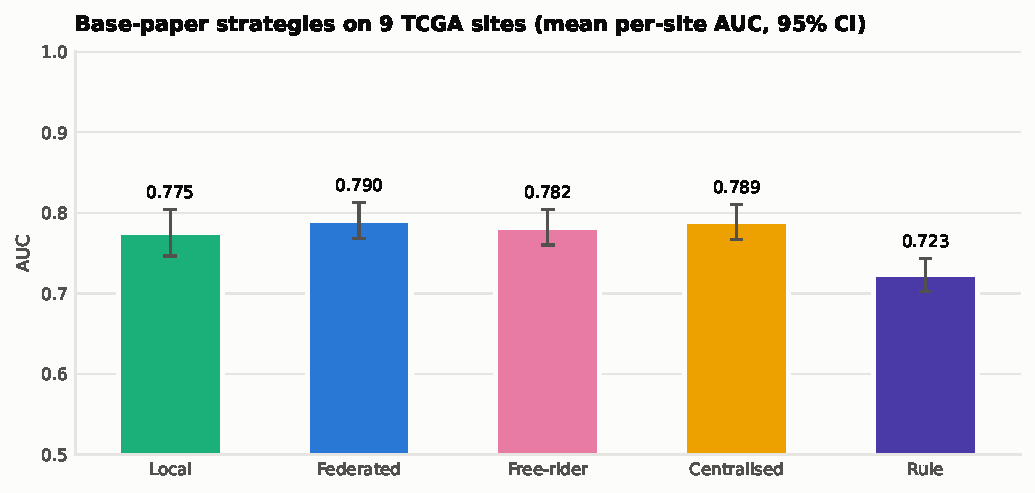
\includegraphics[width=\columnwidth]{figures/figure12_base_paper.pdf}
\caption{Base-paper strategies on the TCGA sites: mean per-site test AUC with 95\% CI over 20 seeds.}
\label{fig:base_paper}
\end{figure}

\begin{figure}[!ht]
\centering
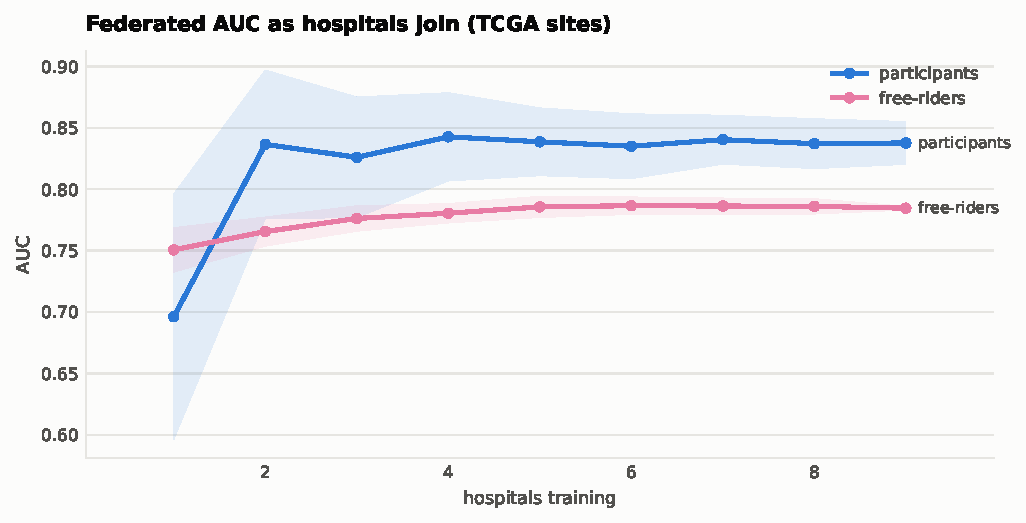
\includegraphics[width=\columnwidth]{figures/figure13_learning_curve.pdf}
\caption{FedAvg AUC for participating sites and for free-riders (non-participating sites and the external small-site pool) as sites join in random order.}
\label{fig:learning_curve}
\end{figure}

\subsection{Centralised Baselines and Feature Sets}
Table~\ref{tab:centralized} compares feature sets with repeated cross-validation. The full clinical set reaches \cvFull{} with the NumPy model used in federation. Adding the protein principal components \emph{lowers} discrimination (paired difference $\cvProtDiff$), and protein features alone reach only \cvProt{}: with roughly 115 components for \nTrain{} training patients the linear model over-fits. Removing the post-surgical pathology features costs $\cvPreopDiff$ (pre-operative model \cvPreop{}). The remaining experiments therefore use the full clinical feature set; the multimodal and pre-operative variants are reported in the ablation.

\begin{table*}[t]
\caption{Centralised baselines: mean AUC over repeated stratified cross-validation (25 folds, 5$\times$5) on the 347-patient cohort. All preprocessing is fitted inside each training fold.}
\centering\small
\begin{tabular}{lccccc}
\toprule
Model & Clinical (full) & Clinical (pre-op) & Protein only & Full + protein & Pre-op + protein \\
\midrule
NumPy LR (ours) & 0.818 & 0.642 & 0.574 & 0.659 & 0.595 \\
LR (L2) & 0.824 & 0.661 & 0.633 & 0.682 & 0.638 \\
LR (L1) & 0.831 & 0.662 & 0.637 & 0.712 & 0.659 \\
Random forest & 0.803 & 0.644 & 0.599 & 0.782 & 0.627 \\
MLP & 0.792 & 0.670 & 0.599 & 0.664 & 0.623 \\
\bottomrule
\end{tabular}
\label{tab:centralized}
\end{table*}


\subsection{Client Drift under Statistical Heterogeneity (H1)}
Table~\ref{tab:drift} and Fig.~\ref{fig:drift} report client drift (Eq.~\ref{M-eq:drift}). Drift grows with heterogeneity (FedAvg: \driftAvgIID{} at $\alpha=100$ to \driftAvgSkew{} at $\alpha=0.1$), and FedProx reduces it by \driftRedMin--\driftRedMax\% at every $\alpha$, with 95\% CIs far from zero; increasing $\mu$ from 0 to 1 lowers drift monotonically (\driftMuZero{} to \driftMuOne{} at $\alpha=0.5$). H1 is supported. The reduction in drift does not translate into higher test AUC without DP: no paired AUC difference is significant, because the convex logistic objective lets FedAvg reach a good solution regardless.

\begin{table*}[t]
\caption{Client drift $\bar d = \mathrm{mean}_{t,k}\|w_k^t - w^{t-1}\|_2$ without DP (3 clients, 20 seeds, mean $\pm$ sd). Spread = max$-$min T3/T4 rate across clients. Last column: paired FedProx$-$FedAvg test-AUC difference with 95\% CI.}
\centering\small
\begin{tabular}{cccccc}
\toprule
$\alpha$ & Spread & FedAvg drift & FedProx drift & Reduction \% [95\% CI] & $\Delta$AUC [95\% CI] \\
\midrule
100 & 0.07 & $0.206 \pm 0.023$ & $0.140 \pm 0.013$ & $32.0$ [31.4, 32.5] & $+0.0022\ [\ensuremath{-}0.0012, +0.0057]$ \\
10 & 0.20 & $0.263 \pm 0.053$ & $0.175 \pm 0.033$ & $33.2$ [32.6, 33.8] & $+0.0018\ [\ensuremath{-}0.0013, +0.0049]$ \\
1 & 0.55 & $0.525 \pm 0.157$ & $0.337 \pm 0.096$ & $35.6$ [34.9, 36.2] & $+0.0019\ [\ensuremath{-}0.0009, +0.0046]$ \\
0.5 & 0.68 & $0.599 \pm 0.165$ & $0.382 \pm 0.100$ & $36.0$ [35.5, 36.5] & $+0.0016\ [\ensuremath{-}0.0024, +0.0056]$ \\
0.1 & 0.84 & $0.770 \pm 0.181$ & $0.488 \pm 0.110$ & $36.4$ [35.9, 36.9] & $+0.0018\ [\ensuremath{-}0.0009, +0.0044]$ \\
\bottomrule
\end{tabular}
\label{tab:drift}
\end{table*}


\begin{figure}[!ht]
\centering
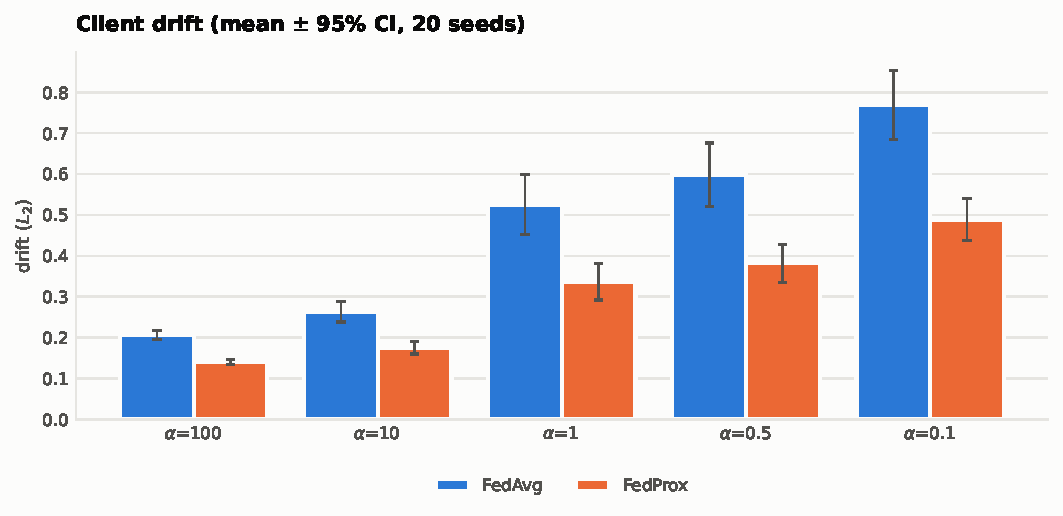
\includegraphics[width=\columnwidth]{figures/figure5_drift.pdf}
\caption{Client drift (Eq.~\ref{M-eq:drift}) of FedAvg and FedProx across Dirichlet $\alpha$ (mean and 95\% CI over 20 seeds).}
\label{fig:drift}
\end{figure}

\subsection{Privacy--Utility Trade-off (H2)}
Fig.~\ref{fig:privacy_utility} shows global test AUC against the privacy budget at $\alpha=10$. Without DP FedAvg reaches \auNoDP{}. Weak privacy is almost free ($\varepsilon=10$: \auAvgTen{}, paired loss $\auLossTen$), whereas strong privacy is costly ($\varepsilon=2$: $\auLossTwo$; $\varepsilon=1$: $\auLossOne$; $\varepsilon=0.5$: $\auLossHalf$). With 20 paired seeds the degradation at $\varepsilon \le 2$ is significant, supporting H2.

\begin{figure}[!ht]
\centering
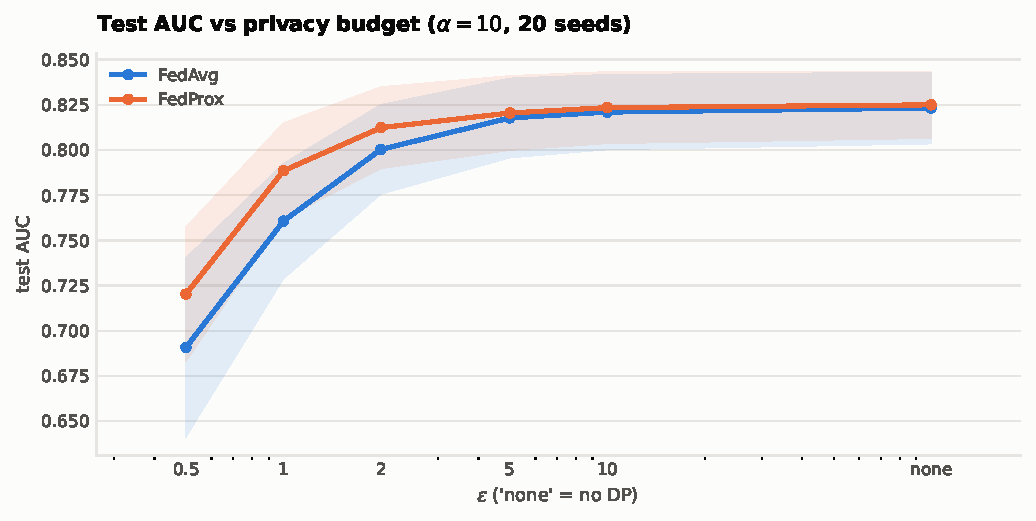
\includegraphics[width=\columnwidth]{figures/figure3_privacy_utility.pdf}
\caption{Global test AUC versus privacy budget $\varepsilon$ ($\alpha=10$, $K=3$; mean and 95\% CI over 20 seeds).}
\label{fig:privacy_utility}
\end{figure}

\subsection{FedProx under Joint Privacy and Heterogeneity (H3)}
Table~\ref{tab:interaction} and Fig.~\ref{fig:heatmap} cross label skew with privacy. Without DP, FedProx and FedAvg are indistinguishable (largest mean difference \gridNoDPmax). Under DP, FedProx is significantly better in \gridSup{} of \gridCells{} cells, by \gridOneHalfMin--\gridOneHalfMax{} AUC at $\varepsilon \in \{1, 0.5\}$, largely independent of $\alpha$. A step-size control explains this: a FedAvg run with half the learning rate matches FedProx (FedProx better in only \gridSupCtl{} of \gridCells{} cells; largest mean difference \gridCtlOneHalfMax{} at $\varepsilon \le 1$). Under DP the proximal term acts mainly as a smaller effective step that damps the injected noise, rather than as a correction for heterogeneity. H3 is therefore supported only in this qualified sense.

\begin{table*}[t]
\caption{Global test AUC under joint label skew ($\alpha$) and privacy ($\varepsilon$), 3 clients, mean over 20 seeds. FedAvg ($\eta/2$) is a step-size control. $\Delta$ = paired FedProx$-$FedAvg difference; bold = 95\% CI excludes 0.}
\centering\small
\begin{tabular}{llcccccc}
\toprule
 & Model & no DP & $\varepsilon=10$ & $\varepsilon=5$ & $\varepsilon=2$ & $\varepsilon=1$ & $\varepsilon=0.5$ \\
\midrule
$\alpha=10$ & FedAvg & 0.823 & 0.821 & 0.818 & 0.800 & 0.761 & 0.691 \\
 & FedProx & 0.825 & 0.823 & 0.821 & 0.812 & 0.789 & 0.720 \\
 & FedAvg ($\eta/2$) & 0.826 & 0.821 & 0.820 & 0.812 & 0.786 & 0.718 \\
 & $\Delta$ Prox$-$Avg & -- & +0.002 & +0.003 & \textbf{+0.012} & \textbf{+0.028} & \textbf{+0.029} \\
\midrule
$\alpha=1$ & FedAvg & 0.823 & 0.821 & 0.818 & 0.801 & 0.757 & 0.688 \\
 & FedProx & 0.825 & 0.823 & 0.820 & 0.812 & 0.787 & 0.717 \\
 & FedAvg ($\eta/2$) & 0.825 & 0.821 & 0.820 & 0.812 & 0.786 & 0.715 \\
 & $\Delta$ Prox$-$Avg & -- & +0.002 & +0.002 & \textbf{+0.012} & \textbf{+0.030} & \textbf{+0.029} \\
\midrule
$\alpha=0.5$ & FedAvg & 0.824 & 0.821 & 0.818 & 0.799 & 0.758 & 0.687 \\
 & FedProx & 0.826 & 0.823 & 0.820 & 0.811 & 0.787 & 0.715 \\
 & FedAvg ($\eta/2$) & 0.826 & 0.821 & 0.820 & 0.811 & 0.784 & 0.715 \\
 & $\Delta$ Prox$-$Avg & -- & +0.002 & +0.002 & \textbf{+0.012} & \textbf{+0.029} & \textbf{+0.028} \\
\midrule
$\alpha=0.1$ & FedAvg & 0.825 & 0.821 & 0.818 & 0.796 & 0.753 & 0.684 \\
 & FedProx & 0.826 & 0.823 & 0.820 & 0.809 & 0.782 & 0.713 \\
 & FedAvg ($\eta/2$) & 0.827 & 0.821 & 0.820 & 0.810 & 0.782 & 0.712 \\
 & $\Delta$ Prox$-$Avg & -- & +0.002 & +0.002 & \textbf{+0.012} & \textbf{+0.029} & \textbf{+0.029} \\
\bottomrule
\end{tabular}
\label{tab:interaction}
\end{table*}


\begin{figure}[!ht]
\centering
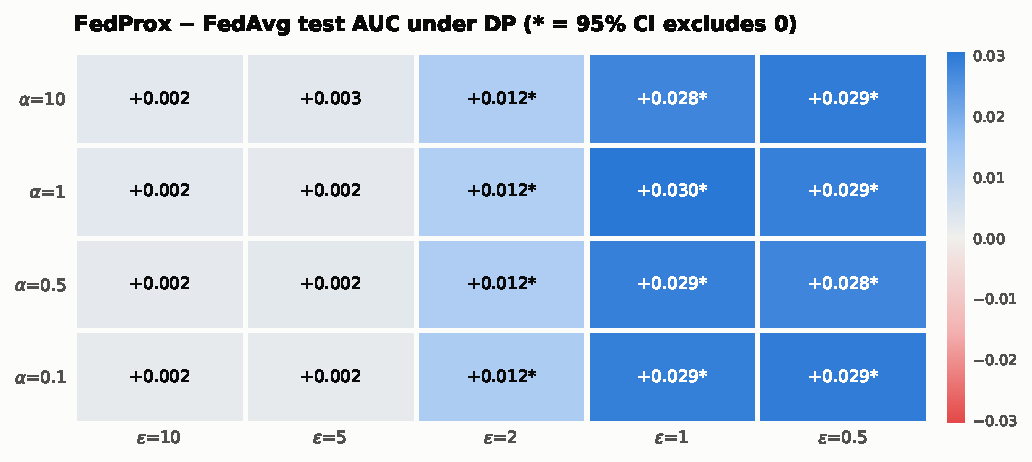
\includegraphics[width=\columnwidth]{figures/figure4_heatmap.pdf}
\caption{Paired FedProx$-$FedAvg test-AUC difference across $\alpha$ and $\varepsilon$ (20 seeds; * = 95\% CI excludes 0).}
\label{fig:heatmap}
\end{figure}

\subsection{Personalised Adaptation (H4)}
Table~\ref{tab:local_adaptation} and Fig.~\ref{fig:pfl} evaluate each client on its own test split ($\alpha=0.5$). With three clients, FedProx reaches \pflProxThree{} per client against \pflLocalThree{} for local-only models, and personalised fine-tuning (PFL) reaches \pflPFLThree{} (PFL$-$Local $=\pflGainThree$). PFL does not improve on the global FedProx model (PFL$-$FedProx $=\pflVsProxThree$ for $K=3$, $\pflVsProxTen$ for $K=10$). With $K=10$ the comparison is again in favour of collaboration (PFL$-$Local $=\pflGainTen$). Because many clients have a single-class test split under strong skew, these averages cover only the clients with a defined AUC (Table~\ref{tab:local_adaptation}). H4 is supported for PFL versus local training, but not for PFL versus the global model.

\begin{table*}[t]
\caption{Mean per-client test AUC ($\alpha=0.5$, 20 seeds) over clients whose local test split contains both classes (\#def. = mean number of such clients). PFL = proximal fine-tuning of the FedProx model. Paired differences with 95\% CI.}
\centering\small
\begin{tabular}{ccccccrr}
\toprule
$K$ & \#def. & Local & FedAvg & FedProx & PFL & PFL$-$Local & PFL$-$FedProx \\
\midrule
3 & 2.2 & 0.754 & 0.810 & 0.811 & 0.805 & $+0.051\ [+0.015, +0.086]$ & $-0.006\ [\ensuremath{-}0.022, +0.011]$ \\
5 & 2.9 & 0.796 & 0.820 & 0.817 & 0.814 & $+0.018\ [\ensuremath{-}0.021, +0.057]$ & $-0.003\ [\ensuremath{-}0.011, +0.005]$ \\
10 & 3.5 & 0.785 & 0.840 & 0.841 & 0.838 & $+0.053\ [+0.010, +0.096]$ & $-0.003\ [\ensuremath{-}0.014, +0.007]$ \\
\bottomrule
\end{tabular}
\label{tab:local_adaptation}
\end{table*}


\begin{figure}[!ht]
\centering
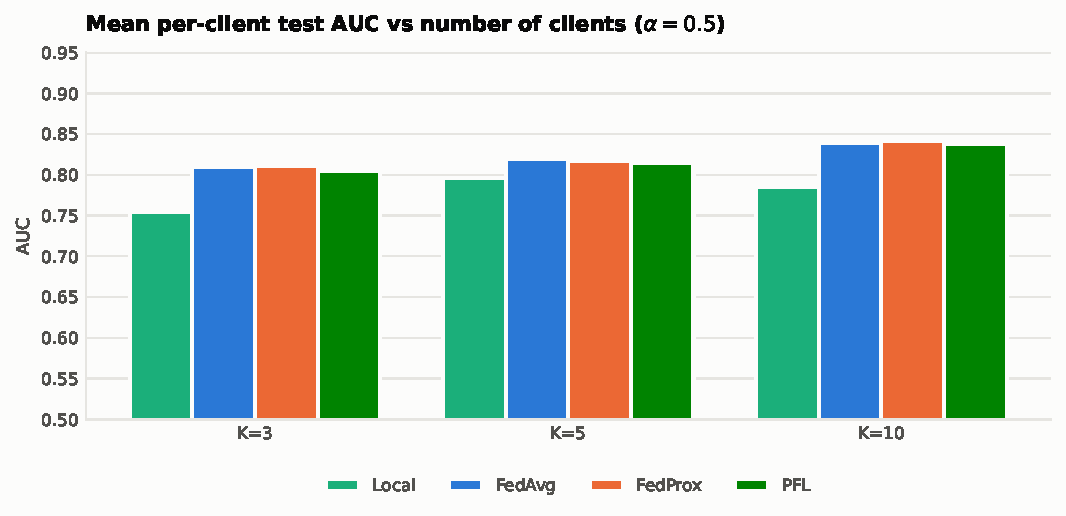
\includegraphics[width=\columnwidth]{figures/figure10_fedprox_scaling_benefit.pdf}
\caption{Mean per-client test AUC of local, FedAvg, FedProx and personalised models for $K \in \{3, 5, 10\}$ clients ($\alpha=0.5$, 20 seeds).}
\label{fig:pfl}
\end{figure}

\subsection{Contribution Valuation under Privacy Noise (H5)}
\label{sec:contribution_valuation}
Without DP, exact Shapley values are positive for every client and track client size only moderately (Spearman with size: \shSizeThree{} for $K=3$, \shSizeTen{} for $K=10$); LOO rankings agree with Shapley rankings only partially (\shLooThree{} for $K=3$, \shLooTen{} for $K=10$), because LOO ignores sub-coalitions and becomes nearly zero when one client is redundant.

Table~\ref{tab:wilcoxon_results} and Figs.~\ref{fig:shapley_instability}--\ref{fig:shapley_scaling_instability} quantify how DP changes these values. Each DP realisation is compared with the no-DP ranking of the same partition, so the Shapley computation itself contributes no randomness (exact enumeration). Rank agreement falls monotonically as privacy strengthens: for $K=3$, Spearman $\rho$ drops from \shRhoTenThree{} at $\varepsilon=10$ to \shRhoHalfThree{} at $\varepsilon=0.5$, and for $K=10$ from \shRhoTenTen{} to \shRhoHalfTen{}. Even the weakest budget leaves $\rho$ well below 0.90 (one-sided Wilcoxon $p<0.01$ in every configuration). The probability that the no-DP top contributor is still ranked first falls from \shTSTenThree{} to \shTSHalfThree{} for $K=3$ (chance 0.33) and from \shTSTenTen{} to \shTSHalfTen{} for $K=10$ (chance 0.10), and at $\varepsilon=0.5$ the rank-reversal rate reaches \shRRHalfTen{} for $K=10$. The overall rank correlation degrades by a similar amount for every federation size, whereas exact ranks and the top contributor are least stable in larger federations. H5 is supported: an incentive scheme that pays hospitals according to Shapley values computed from DP-trained models would frequently reward the wrong hospital.

\begin{table*}[t]
\caption{Stability of exact Shapley rankings under DP relative to the no-DP ranking (20 partitions; 5, 5, 2 noise realisations per partition for $K=3, 5, 10$). TS = probability that the no-DP top contributor is still ranked first (chance = $1/K$). $p$: one-sided Wilcoxon test of $\rho-0.90<0$.}
\centering\small
\begin{tabular}{ccccccc}
\toprule
$K$ & $\varepsilon$ & Spearman $\rho$ [95\% CI] & Rank reversal & TS & Chance TS & $p$ \\
\midrule
3 & 10 & 0.68 [0.50, 0.85] & 0.30 & 0.79 & 0.33 & 0.007 \\
3 & 5 & 0.54 [0.35, 0.73] & 0.38 & 0.73 & 0.33 & 4.1e-4 \\
3 & 2 & 0.40 [0.21, 0.60] & 0.48 & 0.61 & 0.33 & 1.4e-4 \\
3 & 1 & 0.36 [0.16, 0.56] & 0.51 & 0.56 & 0.33 & 6.4e-5 \\
3 & 0.5 & 0.25 [0.07, 0.43] & 0.57 & 0.51 & 0.33 & 4.3e-5 \\
\midrule
5 & 10 & 0.66 [0.55, 0.78] & 0.52 & 0.65 & 0.20 & 7.0e-5 \\
5 & 5 & 0.59 [0.45, 0.72] & 0.59 & 0.60 & 0.20 & 5.1e-5 \\
5 & 2 & 0.46 [0.30, 0.62] & 0.66 & 0.48 & 0.20 & 4.4e-5 \\
5 & 1 & 0.37 [0.21, 0.52] & 0.73 & 0.40 & 0.20 & 4.4e-5 \\
5 & 0.5 & 0.30 [0.15, 0.45] & 0.74 & 0.41 & 0.20 & 4.4e-5 \\
\midrule
10 & 10 & 0.73 [0.67, 0.79] & 0.76 & 0.62 & 0.10 & 5.2e-5 \\
10 & 5 & 0.66 [0.58, 0.75] & 0.77 & 0.60 & 0.10 & 9.5e-7 \\
10 & 2 & 0.55 [0.45, 0.64] & 0.79 & 0.45 & 0.10 & 4.4e-5 \\
10 & 1 & 0.48 [0.39, 0.56] & 0.82 & 0.38 & 0.10 & 4.4e-5 \\
10 & 0.5 & 0.36 [0.26, 0.47] & 0.88 & 0.30 & 0.10 & 4.4e-5 \\
\bottomrule
\end{tabular}
\label{tab:wilcoxon_results}
\end{table*}


\begin{figure}[!ht]
\centering
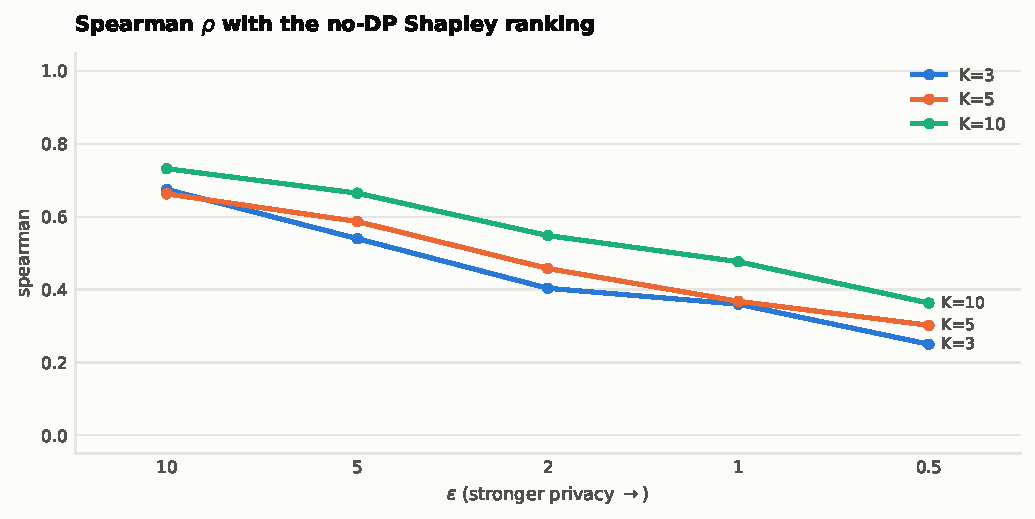
\includegraphics[width=\columnwidth]{figures/figure9_shapley_instability.pdf}
\caption{Spearman correlation between DP and no-DP exact Shapley rankings versus $\varepsilon$ for $K \in \{3, 5, 10\}$ clients (20 partitions).}
\label{fig:shapley_instability}
\end{figure}

\begin{figure}[!ht]
\centering
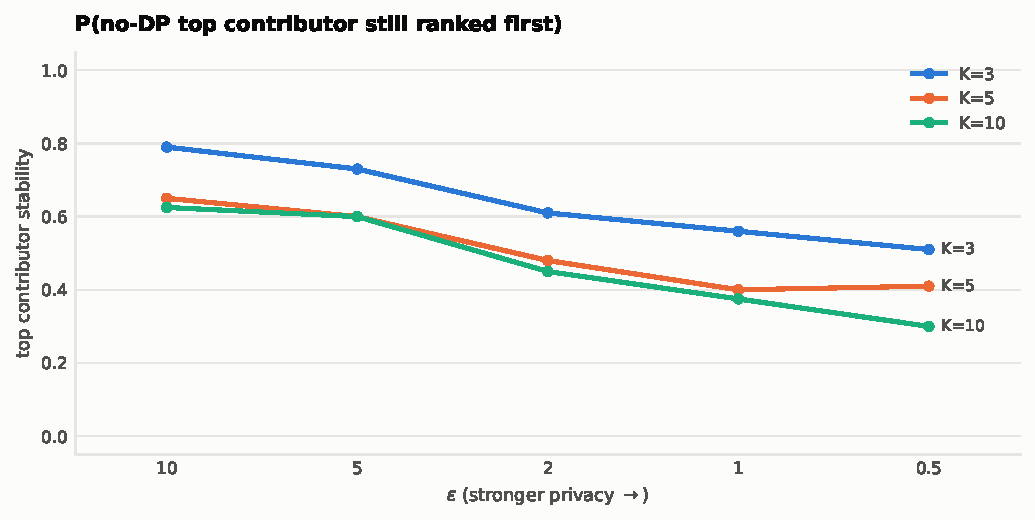
\includegraphics[width=\columnwidth]{figures/figure11_shapley_scaling_instability.pdf}
\caption{Top-contributor stability (probability that the no-DP top contributor stays first under DP) versus $\varepsilon$; chance level is $1/K$.}
\label{fig:shapley_scaling_instability}
\end{figure}

\begin{figure}[!ht]
\centering
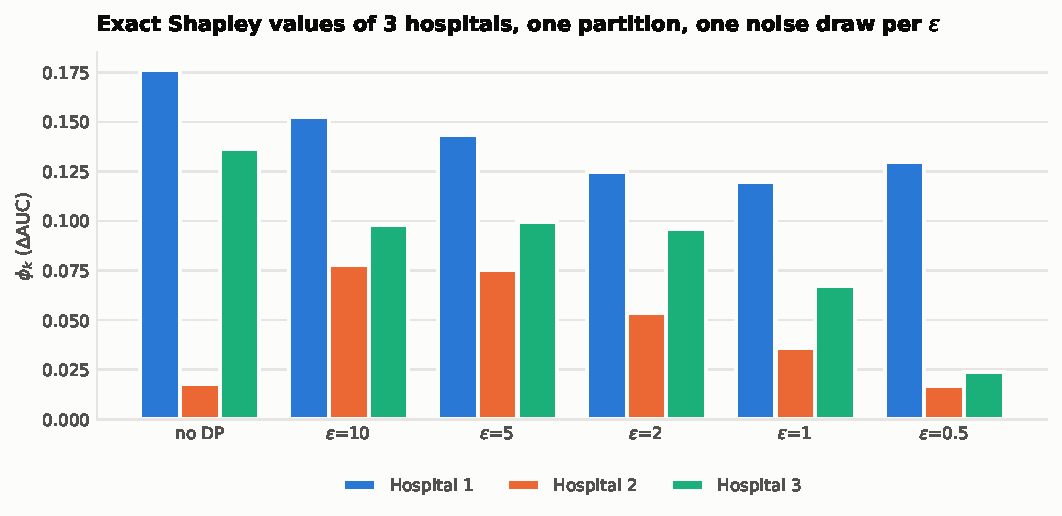
\includegraphics[width=\columnwidth]{figures/figure6_shapley.pdf}
\caption{Exact Shapley values of three clients for one partition: no DP and one DP noise draw per $\varepsilon$.}
\label{fig:shapley_volatility}
\end{figure}

\subsection{Empirical Membership-Inference Evaluation (H7)}
Without DP the confidence-threshold attack is at chance level (attack AUC $\miaNoDP$), and it stays there under DP ($\varepsilon=1$: $\miaOne$; $\varepsilon=0.5$: $\miaHalf$). The positive control confirms that the attack works when a model memorises its training data (AUC $\miaCtl$). The 18-feature logistic model generalises well (train$-$test AUC gap $\miaGap$), so there is little membership signal for DP to remove. The formal DP guarantee still holds, but its \emph{empirical} benefit cannot be demonstrated with this attack, and H7 is not supported. (The previously reported reduction from 0.568 to 0.480 arose in a pipeline whose identifier features let the model memorise individual patients.)

\begin{figure}[!ht]
\centering
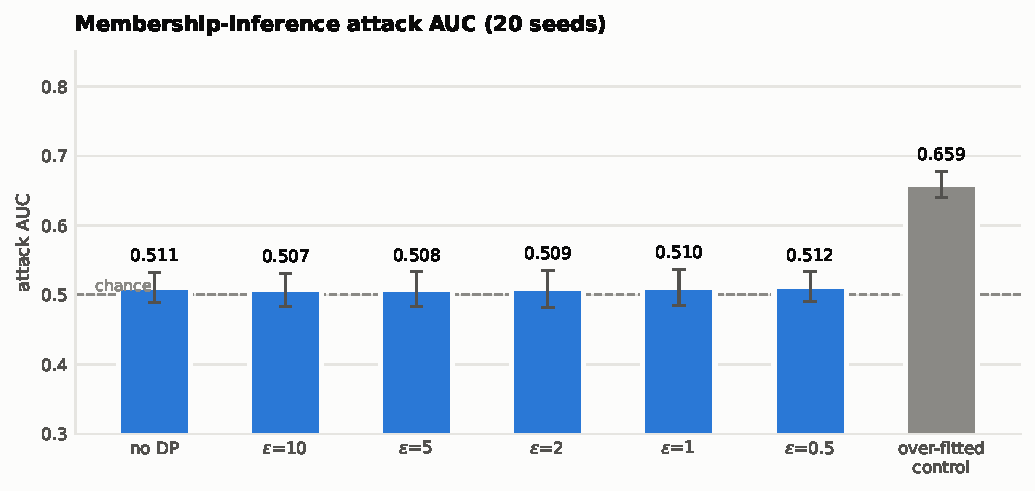
\includegraphics[width=\columnwidth]{figures/figure7_mia.pdf}
\caption{Membership-inference attack AUC (mean and 95\% CI over 20 seeds) without DP, under DP, and for an over-fitted positive control. 0.5 = chance.}
\label{fig:mia}
\end{figure}

\subsection{Controlled Distribution-Shift Stress Test (H6)}
Under synthetic covariate shift the FedProx model degrades gracefully (AUC \shiftBase{} $\to$ \shiftCovTwo{} at severity 2), while concept shift, which flips labels, drives it to \shiftConTwo{} (Fig.~\ref{fig:stress_test}). This is a sensitivity analysis on perturbed copies of the test split, not an external validation.

\begin{figure}[!ht]
\centering
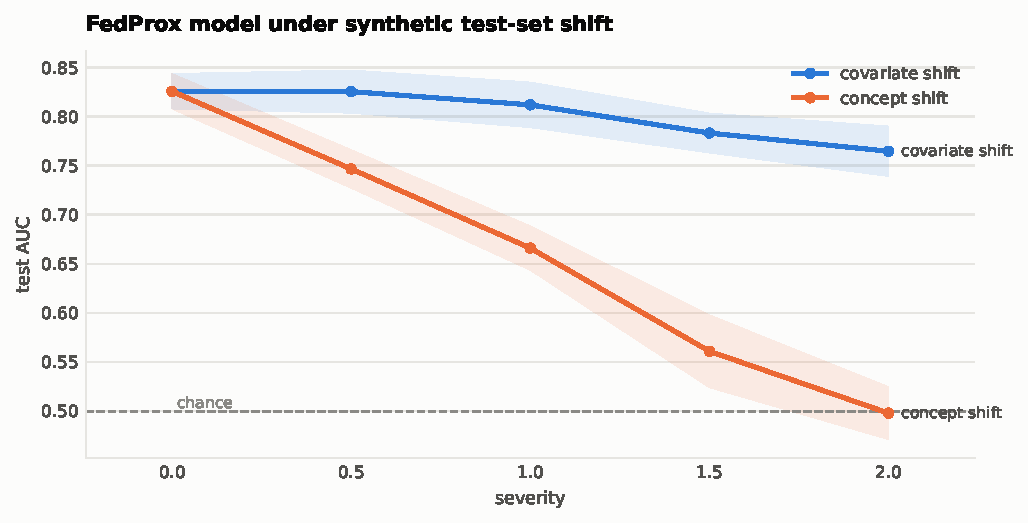
\includegraphics[width=\columnwidth]{figures/figure8_stress_test.pdf}
\caption{FedProx test AUC under synthetic covariate and concept shift of the test split (20 seeds).}
\label{fig:stress_test}
\end{figure}

\subsection{Ablation}
Table~\ref{tab:global_ablation} summarises the components on the global test split ($K=3$, $\alpha=0.5$). FedAvg (\abAvg{}) and FedProx (\abProx{}) match centralised training (\abCen{}). DP costs little at $\varepsilon=5$ (\abDPFive{}) and more at $\varepsilon=1$ (\abDPOne{}). Using only pre-operative features (\abPreop{}) or adding protein components (\abProt{}) both reduce discrimination substantially.

\begin{table}[t]
\caption{Ablation on the global test split ($K=3$, $\alpha=0.5$, 20 seeds, mean $\pm$ sd; paired difference to FedProx with 95\% CI).}
\centering\scriptsize
\setlength{\tabcolsep}{4pt}
\begin{tabular}{p{2.9cm}cc}
\toprule
Configuration & Test AUC & vs FedProx \\
\midrule
Centralised (pooled data) & $0.823 \pm 0.042$ & $-0.003\ [\ensuremath{-}0.008, +0.002]$ \\
FedAvg & $0.824 \pm 0.041$ & $-0.002\ [\ensuremath{-}0.006, +0.002]$ \\
FedProx & $0.826 \pm 0.038$ & reference \\
FedProx + DP ($\varepsilon$=5) & $0.820 \pm 0.045$ & $-0.006\ [\ensuremath{-}0.012, +0.001]$ \\
FedProx + DP ($\varepsilon$=1) & $0.787 \pm 0.058$ & $-0.039\ [\ensuremath{-}0.056, \ensuremath{-}0.022]$ \\
FedProx: pre-op features only & $0.659 \pm 0.062$ & $-0.167\ [\ensuremath{-}0.193, \ensuremath{-}0.141]$ \\
FedProx: clinical (full) + protein PCs & $0.682 \pm 0.050$ & $-0.144\ [\ensuremath{-}0.166, \ensuremath{-}0.122]$ \\
\bottomrule
\end{tabular}
\label{tab:global_ablation}
\end{table}


\section{Survival Analysis Limitation}
A federated Cox model was implemented, but the matched cohort contains only \nEvents{} deaths among \nMatched{} patients (\nEventsTest{} in the reference test split), so out-of-sample survival discrimination cannot be estimated reliably. No survival claims are made.


\section{Detailed PCa-19 Tables}
This section collects the detailed tables of the PCa-19 evaluation referred to in the main text.

\begin{table}[t]
\caption{PCa-19: the base paper's 19-hospital pre-biopsy cohort (5{,}610 men). csPCa = ISUP grade group $\geq 2$ at biopsy; medians of age (years), PSA (ng/mL) and prostate volume (mL); PI-RADS $\geq 4$ in \%.}
\centering\scriptsize
\setlength{\tabcolsep}{3pt}
\begin{tabular}{llrrrrrr}
\toprule
Hosp. & Country & $n$ & csPCa\% & Age & PSA & Vol. & PI-RADS$\geq$4 \\
\midrule
de1 & Germany & 763 & 43 & 65 & 8.0 & 47 & 74 \\
es7 & Spain & 711 & 50 & 67 & 7.6 & 53 & 55 \\
kr2 & South Korea & 590 & 38 & 68 & 7.0 & 42 & 72 \\
ch2 & China & 530 & 33 & 67 & 10.3 & 41 & 42 \\
kr1 & South Korea & 406 & 25 & 64 & 6.8 & 36 & 28 \\
es6 & Spain & 346 & 43 & 69 & 7.6 & 52 & 78 \\
ch1 & China & 312 & 27 & 66 & 9.7 & 45 & 43 \\
us2 & USA & 310 & 48 & 65 & 7.3 & 46 & 82 \\
us1 & USA & 280 & 45 & 62 & 5.5 & 45 & 62 \\
nl & Netherlands & 266 & 26 & 67 & 11.1 & 56 & 36 \\
it & Italy & 218 & 12 & 65 & 8.0 & 54 & 38 \\
es4 & Spain & 200 & 34 & 69 & 7.6 & 55 & 56 \\
es5 & Spain & 200 & 47 & 70 & 10.6 & 56 & 80 \\
de2 & Germany & 162 & 47 & 65 & 6.5 & 40 & 70 \\
gb & United Kingdom & 133 & 29 & 64 & 7.6 & 45 & 48 \\
es1 & Spain & 79 & 42 & 69 & 6.3 & 61 & 97 \\
es8 & Spain & 58 & 38 & 70 & 6.5 & 56 & 81 \\
es3 & Spain & 30 & 60 & 69 & 9.0 & 50 & 97 \\
es2 & Spain & 16 & 38 & 64 & 277.0 & 81 & 69 \\
\bottomrule
\end{tabular}
\label{tab:pca19_cohort}
\end{table}

\begin{table*}[t]
\caption{Privacy and drift on the 19 real hospitals (mean per-hospital test AUC, 20 seeds). The last two AUC columns are paired differences with 95\% CI; drift = mean $\|w_k-w^{t-1}\|$.}
\centering\small
\begin{tabular}{lccccccc}
\toprule
$\varepsilon$ & $\sigma$ & FedAvg & FedProx & FedAvg ($\eta/2$) & FedAvg $-$ no DP & FedProx $-$ FedAvg($\eta/2$) & Drift Avg / Prox \\
\midrule
no DP & -- & 0.824 & 0.821 & 0.821 & $--$ & $+0.000\ [\ensuremath{-}0.001, +0.002]$ & 0.33 / 0.23 \\
10 & 5.7 & 0.822 & 0.819 & 0.819 & $-0.002\ [\ensuremath{-}0.007, +0.003]$ & $+0.000\ [\ensuremath{-}0.001, +0.002]$ & 0.35 / 0.24 \\
5 & 10.5 & 0.822 & 0.819 & 0.819 & $-0.002\ [\ensuremath{-}0.007, +0.003]$ & $+0.000\ [\ensuremath{-}0.001, +0.002]$ & 0.48 / 0.33 \\
2 & 25.0 & 0.821 & 0.819 & 0.820 & $-0.003\ [\ensuremath{-}0.007, +0.001]$ & $-0.001\ [\ensuremath{-}0.003, +0.001]$ & 0.91 / 0.61 \\
1 & 49.0 & 0.820 & 0.819 & 0.819 & $-0.004\ [\ensuremath{-}0.008, +0.001]$ & $-0.001\ [\ensuremath{-}0.003, +0.002]$ & 1.69 / 1.13 \\
0.5 & 97.0 & 0.819 & 0.818 & 0.819 & $-0.005\ [\ensuremath{-}0.011, +0.001]$ & $-0.001\ [\ensuremath{-}0.003, +0.001]$ & 3.30 / 2.19 \\
\bottomrule
\end{tabular}
\label{tab:pca19_privacy}
\end{table*}

\begin{table}[t]
\caption{Local recalibration on 20\% of each held-out country, evaluated on the other 80\% (mean over 8 countries and 20 seeds). $|\log$ O/E$|$ = 0 and slope = 1 are ideal; DP rows are FedProx + DP.}
\centering\scriptsize
\setlength{\tabcolsep}{4pt}
\begin{tabular}{llccc}
\toprule
Model & Recalibration & $|\log$ O/E$|$ & Slope & Brier \\
\midrule
FedAvg & none & 0.263 & 1.09 & 0.145 \\
 & intercept & 0.071 & 1.09 & 0.136 \\
 & int.\,+\,slope & 0.074 & 0.99 & 0.138 \\
\midrule
DP $\varepsilon=5$ & none & 0.260 & 0.81 & 0.150 \\
 & intercept & 0.080 & 0.81 & 0.140 \\
 & int.\,+\,slope & 0.074 & 0.99 & 0.140 \\
\midrule
DP $\varepsilon=1$ & none & 0.263 & 0.80 & 0.151 \\
 & intercept & 0.081 & 0.80 & 0.140 \\
 & int.\,+\,slope & 0.074 & 1.00 & 0.140 \\
\midrule
Noh & none & 0.205 & 0.97 & 0.144 \\
 & intercept & 0.075 & 0.97 & 0.137 \\
 & int.\,+\,slope & 0.077 & 0.97 & 0.138 \\
\bottomrule
\end{tabular}
\label{tab:pca19_recal}
\end{table}

\begin{table}[t]
\caption{Stability of Shapley contribution rankings under DP on the real PCa-19 hospitals (20 seeds). $\rho$ = Spearman correlation with the no-DP ranking; Rank rev.\ = share of hospital pairs whose order flips relative to the no-DP ranking; TS = probability that the no-DP top contributor stays first.}
\centering\scriptsize
\begin{tabular}{lcccc}
\toprule
Hospitals & $\varepsilon$ & $\rho$ [95\% CI] & Rank rev. & TS \\
\midrule
10 (exact) & 10 & $0.94\ [0.93, 0.95]$ & 0.44 & 0.75 \\
10 (exact) & 5 & $0.94\ [0.92, 0.95]$ & 0.45 & 0.75 \\
10 (exact) & 2 & $0.91\ [0.90, 0.93]$ & 0.57 & 0.80 \\
10 (exact) & 1 & $0.85\ [0.80, 0.90]$ & 0.64 & 0.70 \\
10 (exact) & 0.5 & $0.64\ [0.56, 0.71]$ & 0.79 & 0.40 \\
19 (stratified) & 5 & $0.90\ [0.87, 0.93]$ & 0.80 & 0.45 \\
19 (stratified) & 1 & $0.76\ [0.71, 0.80]$ & 0.84 & 0.45 \\
\bottomrule
\end{tabular}
\label{tab:pca19_shapley}
\end{table}

\begin{table}[t]
\caption{Poisson subsampling with sampled-Gaussian RDP accounting (FedProx, 20 held-out seeds). $\sigma$ = noise multiplier needed for the stated $\varepsilon$ over the given number of local steps; PCa-19: mean per-hospital AUC (difference to full batch in brackets) and calibration slope.}
\centering\scriptsize
\setlength{\tabcolsep}{3pt}
\begin{tabular}{lccccc}
\toprule
Sampling & $\varepsilon$ & $\sigma$ & Steps & AUC & Slope \\
\midrule
full batch (q=1) & no DP & -- & 100 & 0.811 & 1.08 \\
full batch (q=1) & 10 & 5.7 & 100 & 0.811 & 0.78 \\
full batch (q=1) & 5 & 10.5 & 100 & 0.810 & 0.78 \\
full batch (q=1) & 2 & 25.0 & 100 & 0.810 & 0.77 \\
full batch (q=1) & 1 & 49.0 & 100 & 0.809 & 0.76 \\
full batch (q=1) & 0.5 & 97.0 & 100 & 0.806 & 0.72 \\
\midrule
q=0.3 & no DP & -- & 300 & 0.810 ($-0.001$) & 1.09 \\
q=0.3 & 10 & 3.1 & 300 & 0.810 ($-0.001$) & 0.79 \\
q=0.3 & 5 & 5.6 & 300 & 0.810 ($+0.000$) & 0.79 \\
q=0.3 & 2 & 13.1 & 300 & 0.809 ($-0.001$) & 0.79 \\
q=0.3 & 1 & 25.6 & 300 & 0.810 ($+0.001$) & 0.78 \\
q=0.3 & 0.5 & 50.5 & 300 & 0.809 ($+0.003$) & 0.75 \\
\midrule
q=0.1 & no DP & -- & 1000 & 0.810 ($-0.001$) & 1.08 \\
q=0.1 & 10 & 2.0 & 1000 & 0.810 ($-0.001$) & 0.79 \\
q=0.1 & 5 & 3.5 & 1000 & 0.809 ($-0.000$) & 0.79 \\
q=0.1 & 2 & 8.0 & 1000 & 0.810 ($-0.000$) & 0.78 \\
q=0.1 & 1 & 15.6 & 1000 & 0.809 ($+0.000$) & 0.77 \\
q=0.1 & 0.5 & 30.8 & 1000 & 0.807 ($+0.000$) & 0.73 \\
\bottomrule
\end{tabular}
\label{tab:subsampling}
\end{table}

\begin{table}[t]
\caption{OSA-Shapley robustness on PCa-19 (ten hospitals, 20 held-out seeds). Top: Spearman $\rho$ with the exact non-private ranking. Bottom: share of splits in which a hospital with random training labels (es6) is ranked last (no-DP retraining Shapley: 100\%).}
\centering\scriptsize
\begin{tabular}{lcc}
\toprule
Setting & $\varepsilon=2$ & $\varepsilon=1$ \\
\midrule
Local steps = 10 & 0.84 & 0.81 \\
Local steps = 30 (chosen) & 0.89 & 0.80 \\
Local steps = 60 & 0.90 & 0.72 \\
Reference set 25\% of hospital test data & 0.77 & 0.67 \\
Reference set 50\% of hospital test data & 0.87 & 0.77 \\
\midrule
\multicolumn{3}{l}{\emph{Useless hospital ranked last}} \\
OSA (cost $\varepsilon$) & 100\% & 95\% \\
MR (cost $\varepsilon$) & 70\% & 80\% \\
OR (cost $\varepsilon$) & 100\% & 100\% \\
Retraining, budget-matched (cost $\varepsilon$) & 60\% & 45\% \\
Retraining, per run (true $\varepsilon$ 85 and 33) & 100\% & 100\% \\
\bottomrule
\end{tabular}
\label{tab:osa_robust}
\end{table}


\section{Claims and Computed Verdicts}
\begin{table*}[t]
\caption{Claim--evidence summary. Verdicts are computed from the result files: `supported' only if the 95\% CI of the paired difference over seeds excludes 0 in the claimed direction; the pre-registered rows are scored by the criteria fixed in advance (Section~\ref{sec:prereg}).}
\centering\scriptsize
\begin{tabular}{p{1.4cm}p{4.2cm}p{8.6cm}p{1.5cm}}
\toprule
Area & Claim & Evidence (mean [95\% CI]) & Verdict \\
\midrule
PCa-19 (19 hospitals) & Joining FL gives hospitals a significant average local gain & FL - LOC (mean per-hospital AUC) = \ensuremath{-}0.005 {[}-0.015, +0.006{]} & not significant \\
PCa-19 (19 hospitals) & Free-riders get (almost) the same model as participants & FR - FL = \ensuremath{-}0.002 {[}-0.002, \ensuremath{-}0.001{]} & supported \\
PCa-19 (19 hospitals) & Federated training matches pooled training & CEN - FL = +0.002 {[}-0.001, +0.004{]} & supported \\
PCa-19 (19 hospitals) & FL beats the published Noh calculator (hospital-averaged AUC) & FL - Noh = \ensuremath{-}0.010 {[}-0.016, \ensuremath{-}0.005{]}; patient-weighted FL 0.856 vs Noh 0.850 & opposite \\
PCa-19 (19 hospitals) & Our re-implementation reproduces the base paper's code exactly & noh: max $|$difference$|$ 1.2e-14 over 5x19 cells (50 repeats); ettala: max $|$difference$|$ 7.8e-15 over 5x19 cells (50 repeats) & supported \\
PCa-19 (19 hospitals) & Federated model transports to unseen countries as well as pooled training & leave-one-country-out, FedAvg - centralised = \ensuremath{-}0.000 {[}-0.001, +0.001{]} (8 countries) & supported \\
PCa-19 (19 hospitals) & DP lowers the calibration slope (predictions more extreme) on held-out countries & slope at $\varepsilon$=5 = 0.81 {[}0.70, 0.92{]} over 8 countries (no DP 1.12) & supported \\
PCa-19 (19 hospitals) & Local recalibration (20\% of a new country) fixes calibration-in-the-large & $|$log O/E$|$ recalibrated - transported = \ensuremath{-}0.193 {[}-0.347, \ensuremath{-}0.038{]} & supported \\
PCa-19 (19 hospitals) & Strong privacy ($\varepsilon$ = 0.5) costs $<$ 0.02 AUC at this scale & FedAvg($\varepsilon$=0.5) - no DP = \ensuremath{-}0.005 {[}-0.011, +0.001{]} & supported \\
PCa-19 (19 hospitals) & FedProx's effect equals halving FedAvg's learning rate & largest $|$FedProx - FedAvg(lr/2)$|$ over 6 privacy levels = 0.0009 AUC; drift reduction 30.8\% & explained by step size \\
PCa-19 (19 hospitals) & Personalisation helps small hospitals ($<$ 100 patients) & PFL - FedProx = +0.039 {[}+0.013, +0.065{]} & supported \\
PCa-19 (19 hospitals) & DP noise destabilises Shapley rankings of real hospitals & 10 hospitals: Spearman 0.94 ($\varepsilon$=10) $\rightarrow$ 0.64 ($\varepsilon$=0.5) & supported \\
PCa-19 (19 hospitals) & OSA-Shapley beats retraining at the same real privacy cost ($\varepsilon$ = 2) & Spearman with exact Shapley: OSA - budget-matched retraining = +0.71 {[}+0.58, +0.84{]} & supported \\
PCa-19 (19 hospitals) & OSA-Shapley is not significantly worse than per-run retraining, which spends far more privacy ($\varepsilon$ = 2) & OSA - per-run retraining = \ensuremath{-}0.02 {[}-0.06, +0.03{]} (per-run real $\varepsilon$ = 85) & supported \\
PCa-19 (19 hospitals) & OSA-Shapley beats reconstruction from the DP training run (MR, GTG upper bound) at the same cost ($\varepsilon$ = 2) & OSA - MR = +0.14 {[}+0.08, +0.19{]}; OSA - OR = +0.37 {[}+0.26, +0.48{]} & supported \\
PCa-19 (19 hospitals) & OSA-Shapley ranks a hospital with random labels last more often than budget-matched retraining ($\varepsilon$ = 2) & ranked last: OSA 100\%, MR 70\%, budget-matched retraining 60\% & supported \\
PCa-19 (19 hospitals) & OSA-Shapley beats sharing hospital size (10 largest hospitals, $\varepsilon$ = 2) & OSA - size = +0.80 {[}+0.70, +0.91{]}; rho size 0.08, statistics \ensuremath{-}0.18 & supported \\
PCa-19 (19 hospitals) & OSA-Shapley beats the single-model AUC of the same DP releases (10 largest, $\varepsilon$ = 1) & OSA - single-model AUC = +0.10 {[}+0.05, +0.14{]} ($\varepsilon$ = 1); +0.04 {[}-0.00, +0.08{]} ($\varepsilon$ = 2) & supported \\
PCa-19 (19 hospitals) & On the 10 smallest real hospitals OSA-Shapley beats reconstruction ($\varepsilon$ = 2) & OSA - MR = +0.00 {[}-0.06, +0.06{]}; OSA - size = +0.05 {[}-0.01, +0.10{]} & not significant \\
PCa-19 (19 hospitals) & OSA-Shapley also beats reconstruction with a non-convex model (federated MLP, $\varepsilon$ = 2) & OSA-ensemble - MR = \ensuremath{-}0.17 {[}-0.25, \ensuremath{-}0.09{]} (rho 0.65 vs 0.82) & opposite \\
PCa-19 (19 hospitals) & With an MLP, post-processing valuation beats budget-matched retraining ($\varepsilon$ = 2) & OSA-ensemble - budget-matched = +0.47 {[}-0.34, +1.28{]} on 5 splits; MR 0.80 & not significant \\
PCa-19 (19 hospitals) & A stronger federated algorithm or federated MLP beats converged FedAvg & best: Federated MLP +0.005 {[}+0.001, +0.009{]} vs FedAvg; converged FedAvg (400 steps) +0.002 {[}+0.001, +0.003{]} & not significant \\
PCa-19 (19 hospitals) & Non-linear models (gradient boosting) transport better to unseen countries & leave-one-country-out AUC, gradient boosting - FedAvg = \ensuremath{-}0.003 {[}-0.011, +0.004{]} (8 countries); slope 0.91 & not significant \\
PCa-19 (19 hospitals) & SCAFFOLD reduces client drift more than FedProx without changing AUC & drift FedAvg 0.322, FedProx 0.223, SCAFFOLD 0.113; AUC SCAFFOLD - FedAvg = \ensuremath{-}0.000 {[}-0.001, +0.000{]} & supported \\
PCa-19 (19 hospitals) & Subsampled DP (q = 0.3) improves utility over full batch at $\varepsilon$ = 1 & mean per-hospital AUC difference = +0.001 {[}-0.003, +0.004{]} & not significant \\
Heart (4 hospitals) & Without DP, OSA-Shapley beats reconstruction in a second real federation & OSA - MR = +0.22 {[}+0.05, +0.39{]} (rho 0.92 vs 0.70) & supported \\
Heart (4 hospitals) & Under DP, OSA-Shapley also beats reconstruction in the heart federation ($\varepsilon$ = 2) & OSA - MR = \ensuremath{-}0.30 {[}-0.59, \ensuremath{-}0.01{]} (rho 0.15 vs 0.45); about 43 patients per parameter & opposite \\
Heart (4 hospitals) & Hospital size identifies contributions (no DP) & rho size \ensuremath{-}0.38; OSA - size = +1.30 {[}+1.12, +1.48{]} & not supported \\
Pre-registered rule test & Pre-registered H1: OSA beats MR wherever $\nu$ $\ge$ 100 ($\varepsilon$ = 2) & OSA - MR at $\nu$ = 113: +0.14 {[}+0.08, +0.19{]} & supported \\
Pre-registered rule test & Pre-registered H2: OSA stops beating MR at $\nu$ $\le$ 50 ($\varepsilon$ = 2) & OSA - MR at $\nu$ = 45: +0.18 {[}+0.08, +0.29{]}; $\nu$ = 28: +0.12 {[}+0.00, +0.24{]} & not supported \\
Pre-registered rule test & Pre-registered H3: OSA - MR increases with $\nu$ & Spearman($\nu$, OSA - MR) = 0.57 & supported \\
Pre-registered rule test & Pre-registered H4: the switch-over lies between $\nu$ = 50 and 100 & observed switch-over at $\nu$ = 21 & not supported \\
Pre-registered rule test & Pre-registered H5: fewer patients and more parameters agree at matched $\nu$ & $\nu$ = 45 (fewer patients) +0.18 {[}+0.08, +0.29{]} vs $\nu$ = 40 (more parameters) +0.05 {[}-0.02, +0.12{]} & supported \\
Pre-registered rule test & Pre-registered H6: stronger privacy ($\varepsilon$ = 1) moves the switch-over up & $\varepsilon$ = 1 lower in 5 of 8 conditions; switch-overs at $\nu$ = 26, 29, 38 & supported \\
\bottomrule
\end{tabular}
\label{tab:hyp_summary}
\end{table*}


\bibliographystyle{IEEEtran}
\bibliography{references}
\end{document}
